\documentclass[english]{sbrt}
\usepackage[english]{babel}
\usepackage[utf8]{inputenc}
\usepackage{authblk}
\usepackage{csquotes}
\usepackage{graphicx}
\usepackage{float}
\usepackage{cleveref}
\usepackage{tabularx}
\usepackage[style=apa, natbib=true, backend=biber]{biblatex}
\addbibresource{references.bib}
\newtheorem{theorem}{Teorem}

\begin{document}

\title{Photo/Video Effect Creation on a Person Using Semantic Segmentation}

\author[1*]{Marieta Baghdasaryan}
\author[2*]{Nane Arshakyan}
\author[3**]{Vahagn Hakobyan}
\affil[***]{Capstone Supervisor: Marianna Ohanyan}
\affil[*]{\emph {Bachelor of Science in Computer Science, American University of Armenia}}
\affil[**]{\emph {Bachelor of Science in Data Science, American University of Armenia}}
\affil[1]{marieta\_baghdasaryan@edu.aua.am} 
\affil[2]{nane\_arshakyan@edu.aua.am} 
\affil[3]{vahagn\_hakobyan@edu.aua.am} 

\maketitle

\markboth{PHOTO/VIDEO EFFECT CREATION ON A PERSON USING SEMANTIC SEGMENTATION, 23 MAY 2022, AMERICAN UNIVERSITY OF ARMENIA}{}


\begin{abstract}
Image segmentation has been widely applied in solving computer vision problems, from autonomous vehicles to medical imaging and photo effects. There are different approaches and techniques to image segmentation. However, each one has its specific applications in different use cases. In this work, we present video effects that are created using a semantic segmentation technique that is based on artificial neural networks. The effects include background replacement, RGB glitch, and person outline effect.
\end{abstract}
\begin{keywords}
Semantic segmentation, convolutional neural networks, U-Net
\end{keywords}


\section{Introduction}
With increased number of Big Data applications in businesses, image processing techniques have become crucial for organizing, managing, and making sense of image data. Computer vision is the field of Artificial Intelligence, which is responsible for deriving information from digital visual content. One way to extract information from images is image segmentation. It is a technique used to partition the pixels of the image into different regions and categorize those for further use  (\cite{shapiro_2000_computer}).
Image segmentation applications vary from customer behavior tracking to video surveillance, traffic control systems, and health monitoring, including medical diagnosis, surgery planning, and autonomous driving (\cite{vadapalli_2021_image}). Social media and other visual entertainment and content creation platforms also use image processing. An example of an image processing use case is the implementation of person detection and segmentation techniques for creating visual effects for photography and videography, which will be executed in this project. The widely popular ways of image segmentation are instance segmentation, semantic segmentation, and the recently proposed panoptic segmentation. 
\\ \indent Semantic segmentation is a process that clusters all pixels into classes of an object. One example can classify all people in a photo into one segment and their background into another segment. 
The following process, instance segmentation, identifies and labels each pixel into individual instances of an object. For example, in Fig. 1a and 1b, you can observe an example of semantic segmentation and instance segmentation.

\begin{figure}[hbt]
\centering 
\makebox[\columnwidth]{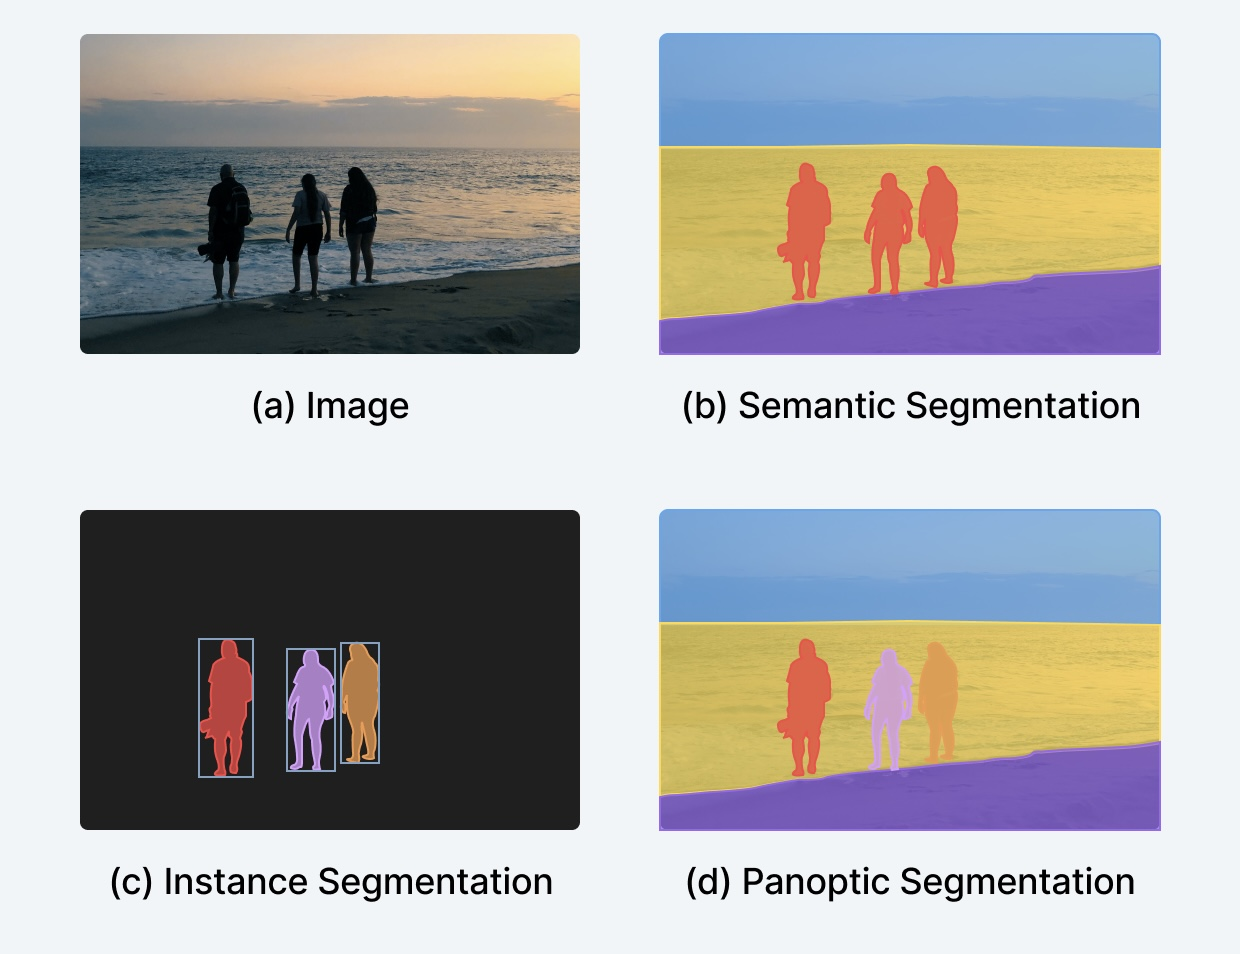
\includegraphics[width=0.5\textwidth]{figures/fig1.jpg}}
\caption{\label{fig:fig1} Visual representation of segmentation approaches: a - the initial version of the image, b - semantic segmentation, c - instance segmentation, and d - panoptic segmentation (\cite{barla_2022_panoptic}).}
\end{figure}

The last approach of image segmentation is panoptic segmentation (Fig. \ref{fig:fig1}d). Each pixel is assigned two labels throughout the segmentation process, their instance and semantic labels (\cite{kirillov_2019_panoptic}). In other words, panoptic segmentation is used to identify and categorize everything on an image, from single objects to uncountable things, like grass, road, etc. This process is mainly used for autonomous driving, medical imaging, and digital image processing. 

\par The typical real-world applications of semantic segmentation have a profound impact across different industries. Semantic segmentation can be used for self-driving cars, retail, and medical scans (\cite{keymakr_2021_instance}). The technique can help an autonomous vehicle's orientation by identifying pedestrians, barriers, other vehicles, and lanes in the first case. On the other hand, the retail industry uses semantic segmentation to suggest to customers similar items based on their choice. This segmentation works perfectly well for digital imagery and photo editing, particularly distinguishing between humans and their backgrounds. One popular use case of semantic segmentation in photo effects can be the portrait mode on the iOS cameras, which use photo segmentation mattes to distinguish between the background and the foreground of an image and thus blur the background (\cite{appleinc_2019_advances}). Throughout this project, the following effects will be created using semantic segmentation: 
\begin{itemize}
    \item Background replacement
    \item RGB glitch effect.
    \item Person outline
\end{itemize}
The code implementation of this project can be found here:
https://github.com/NanehArsh/Capstone.git

\section{Literature Review}
There are two fundamental approaches when it comes to image segmentation. The first approach is similarity detection, and the other one is discontinuity detection. In other words, similarity detection tries to detect similar pixels into a group, combining separate pixels into a region, and the other approach identifies the edges of the regions first through algorithms such as edge detection or line detection. 
Core methods that are used to execute image segmentation are image processing and deep learning methods. The most common techniques used for image segmentation through these methods are the following:  

\begin{itemize}
\item Threshold-based segmentation
\item Edge-based segmentation
\item Region-based segmentation
\item Clustering-based segmentation
\item Neural-networks-based segmentation
\end{itemize}

\noindent The first four methods represent image segmentation techniques, whereas neural-networks-based segmentation is done through deep learning methods.

\subsection{Thresholding-based segmentation}
The image's color space is converted into grayscale when applying this method (\cite{alamri_2010_image}). The segmentation is done by assigning a luminance intensity value to each pixel and dividing the image into two segments based on the threshold value. Although this segmentation technique is quite simple to implement, a thing to consider is that it has poor performance when it comes to the details; they are mostly left out.

\subsection{Edge-based segmentation}
Throughout this process, the edges of the objects are located on an image. The emphasis is on the edges, as they are regarded as the most significant pieces of information on an image (\cite{yuheng_2017_image}). The image size is greatly reduced, and irrelevant information is eliminated from the image. In this case, the image is also being divided into binary segments, one including the pixels that are classified as edges and the other including the rest of the pixels. It classifies the pixels based on the discontinuity of contrasts, textures, luminance, saturation, etc. It is best used when the objects on an image have accentuated contrasts. However, the efficiency drops significantly in noisy images.

\subsection{Region-based segmentation}
This technique of segmentation is based on dividing the image into multiple regions that share similarities, selecting seed pixels for each one of those, and later merging or splitting further the pixel sets that are located around the same neighborhood of pixels, with a seed in the center (\cite{yuheng_2017_image}). Region-based segmentation works pretty well even on noisy images; however, one major drawback is that it requires a lot of memory and time.

\subsection{Clustering-based segmentation}
Clustering-based segmentation locates the pixels with similar features and groups them into specific clusters (\cite{sharma_2020_clusterbased}). These pixels do not have to be neighboring each other. Clustering images into color groups, for example, might help us detect objects that differ from each other by their color. This segmentation technique works pretty well on smaller datasets; however, the computation time might be too large for larger datasets.

\subsection{Neural-networks-based segmentation}
Neural network-based segmentation analyzes and identifies different objects in an image. It is done by training the data on an image dataset to recognize a particular pattern later (\cite{sharif_2010_artificial}). The benefits of this technique are that it is easy to implement, Python libraries are available, and it has practical applications (\cite{prasad_2020_what}). However, training such a model on big datasets might be time-consuming and costly.

\noindent Convolutional neural networks (CNNs) work pretty well with images that have three dimensions. The dimensions are the height, the width, and the RGB value intensity of the image (\cite{kaushik_2019_image}). Based on the benefits of neural network-based segmentation, the project will be executed by implementing a convolutional neural network with a U-Net architecture. 


\begin{figure}[H]
\centering 
\makebox[\columnwidth]{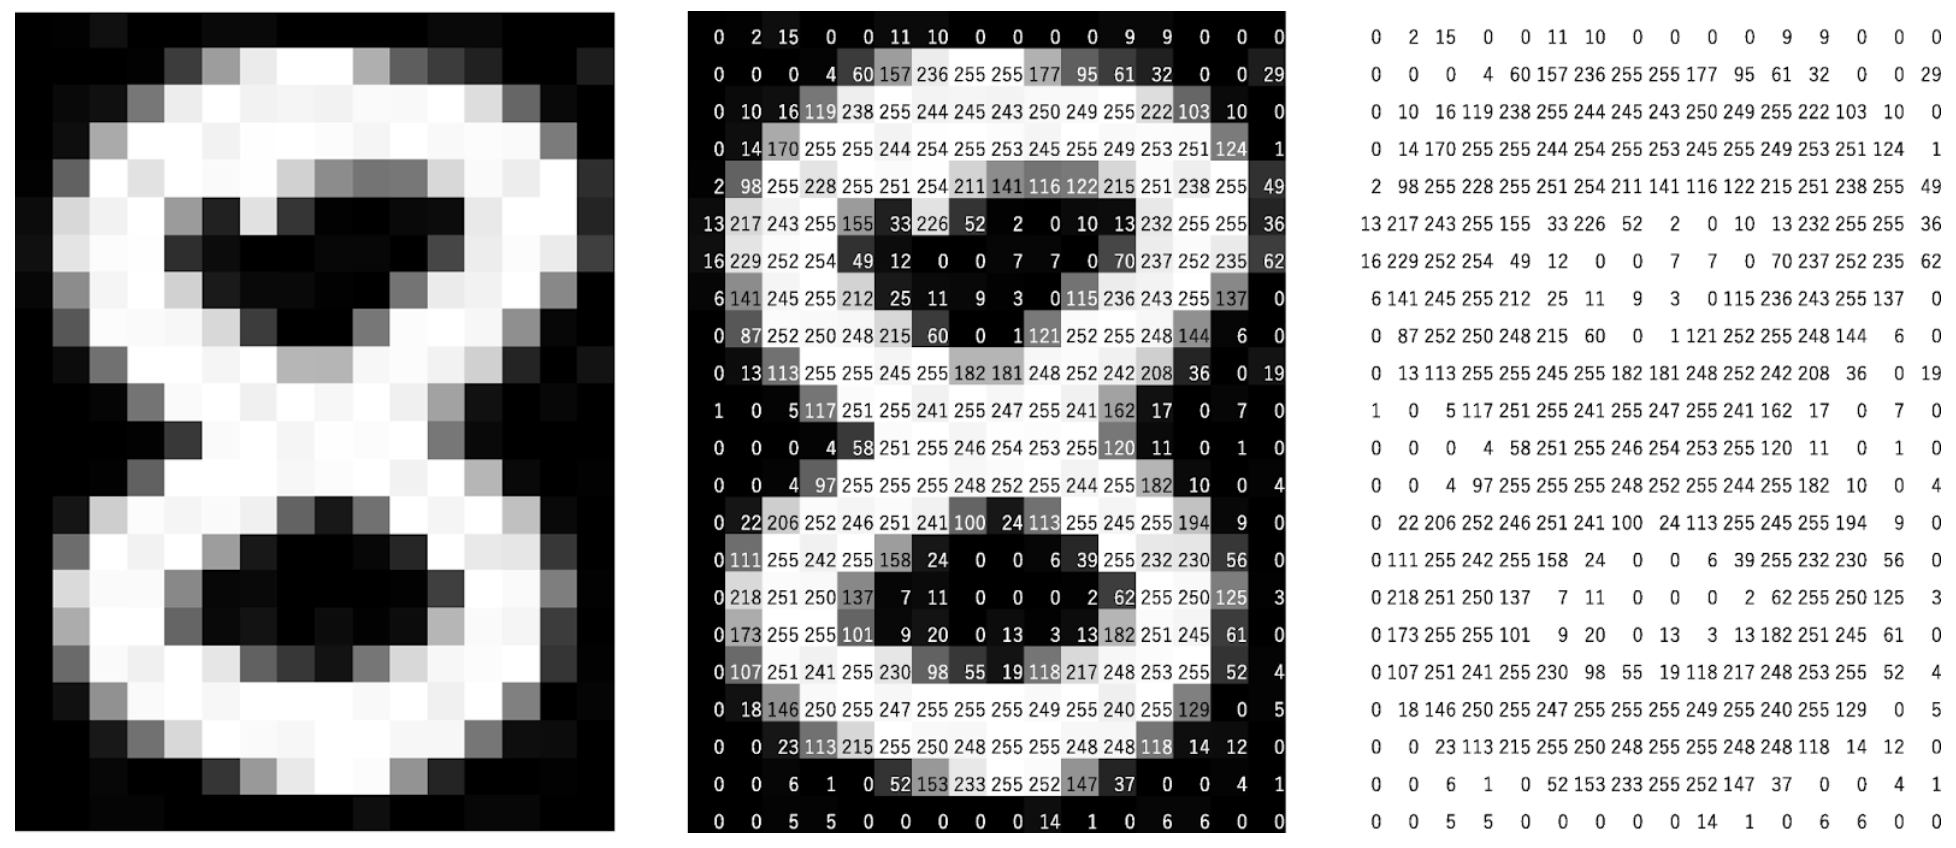
\includegraphics[width=0.5\textwidth]{figures/fig2.png}}
\caption{\label{fig:fig2} The pixelated image on the left, the pixels with their corresponding pixel brightness value in the middle, and the matrix of those values on the right (\cite{yamashita_2018_convolutional}).}
\end{figure}

\section{Prerequisites}
The advances in convolutional neural networks help improve image recognition (\cite{long_2015_fully}). They can be used very effectively in semantic segmentation. The following section highlights the building blocks of CNN that will help to dive deep into the U-Net architecture. 

\par Inspired by the neural networks found within the mammal brain, artificial neural networks consist of neurons and edges. Each neuron takes a signal, processes it, and transmits it to the next neuron via an edge. Each neuron and edge has a weight assigned to it. It signifies the value that each of those carries. Higher weight value corresponds to higher importance of the neuron. The weight, however, continuously changes to fit throughout the learning process of a model to ensure more accurate results. U-Net is such an architecture through which semantic segmentation can be executed (\cite{zhang_2019_unet}). It is a modification of a traditional convolutional neural network introduced to improve biomedical research. It can locate and identify objects in specific regions of an image. It consists of contractive and expansive paths that shape the U-like structure. 


Using this architecture for semantic segmentation is useful, as it labels the pixels that already have their locations marked with their corresponding category value (e.g., person and background). 
A machine can identify an image by using an array of numbers. In an image with a depth of 8 bits, the value of each pixel can take values between 0 and 255 (Visual representation in Fig. \ref{fig:fig2}). For each pixel, there are three color channels: the Red, Green, and Blue channels (RGB), each corresponding value between 0 and 255. The combination of these three channels makes up the colorful images. To represent an image in the form of a matrix, we need a 3-dimensional matrix, having the height and the width of an image as two dimensions and the depth (RGB channels separately) as a third dimension. 


A CNN architecture consists of multiple building blocks, including convolutional layers and pooling layers.  

\begin{figure}[hbt]
\centering 
\makebox[\columnwidth]{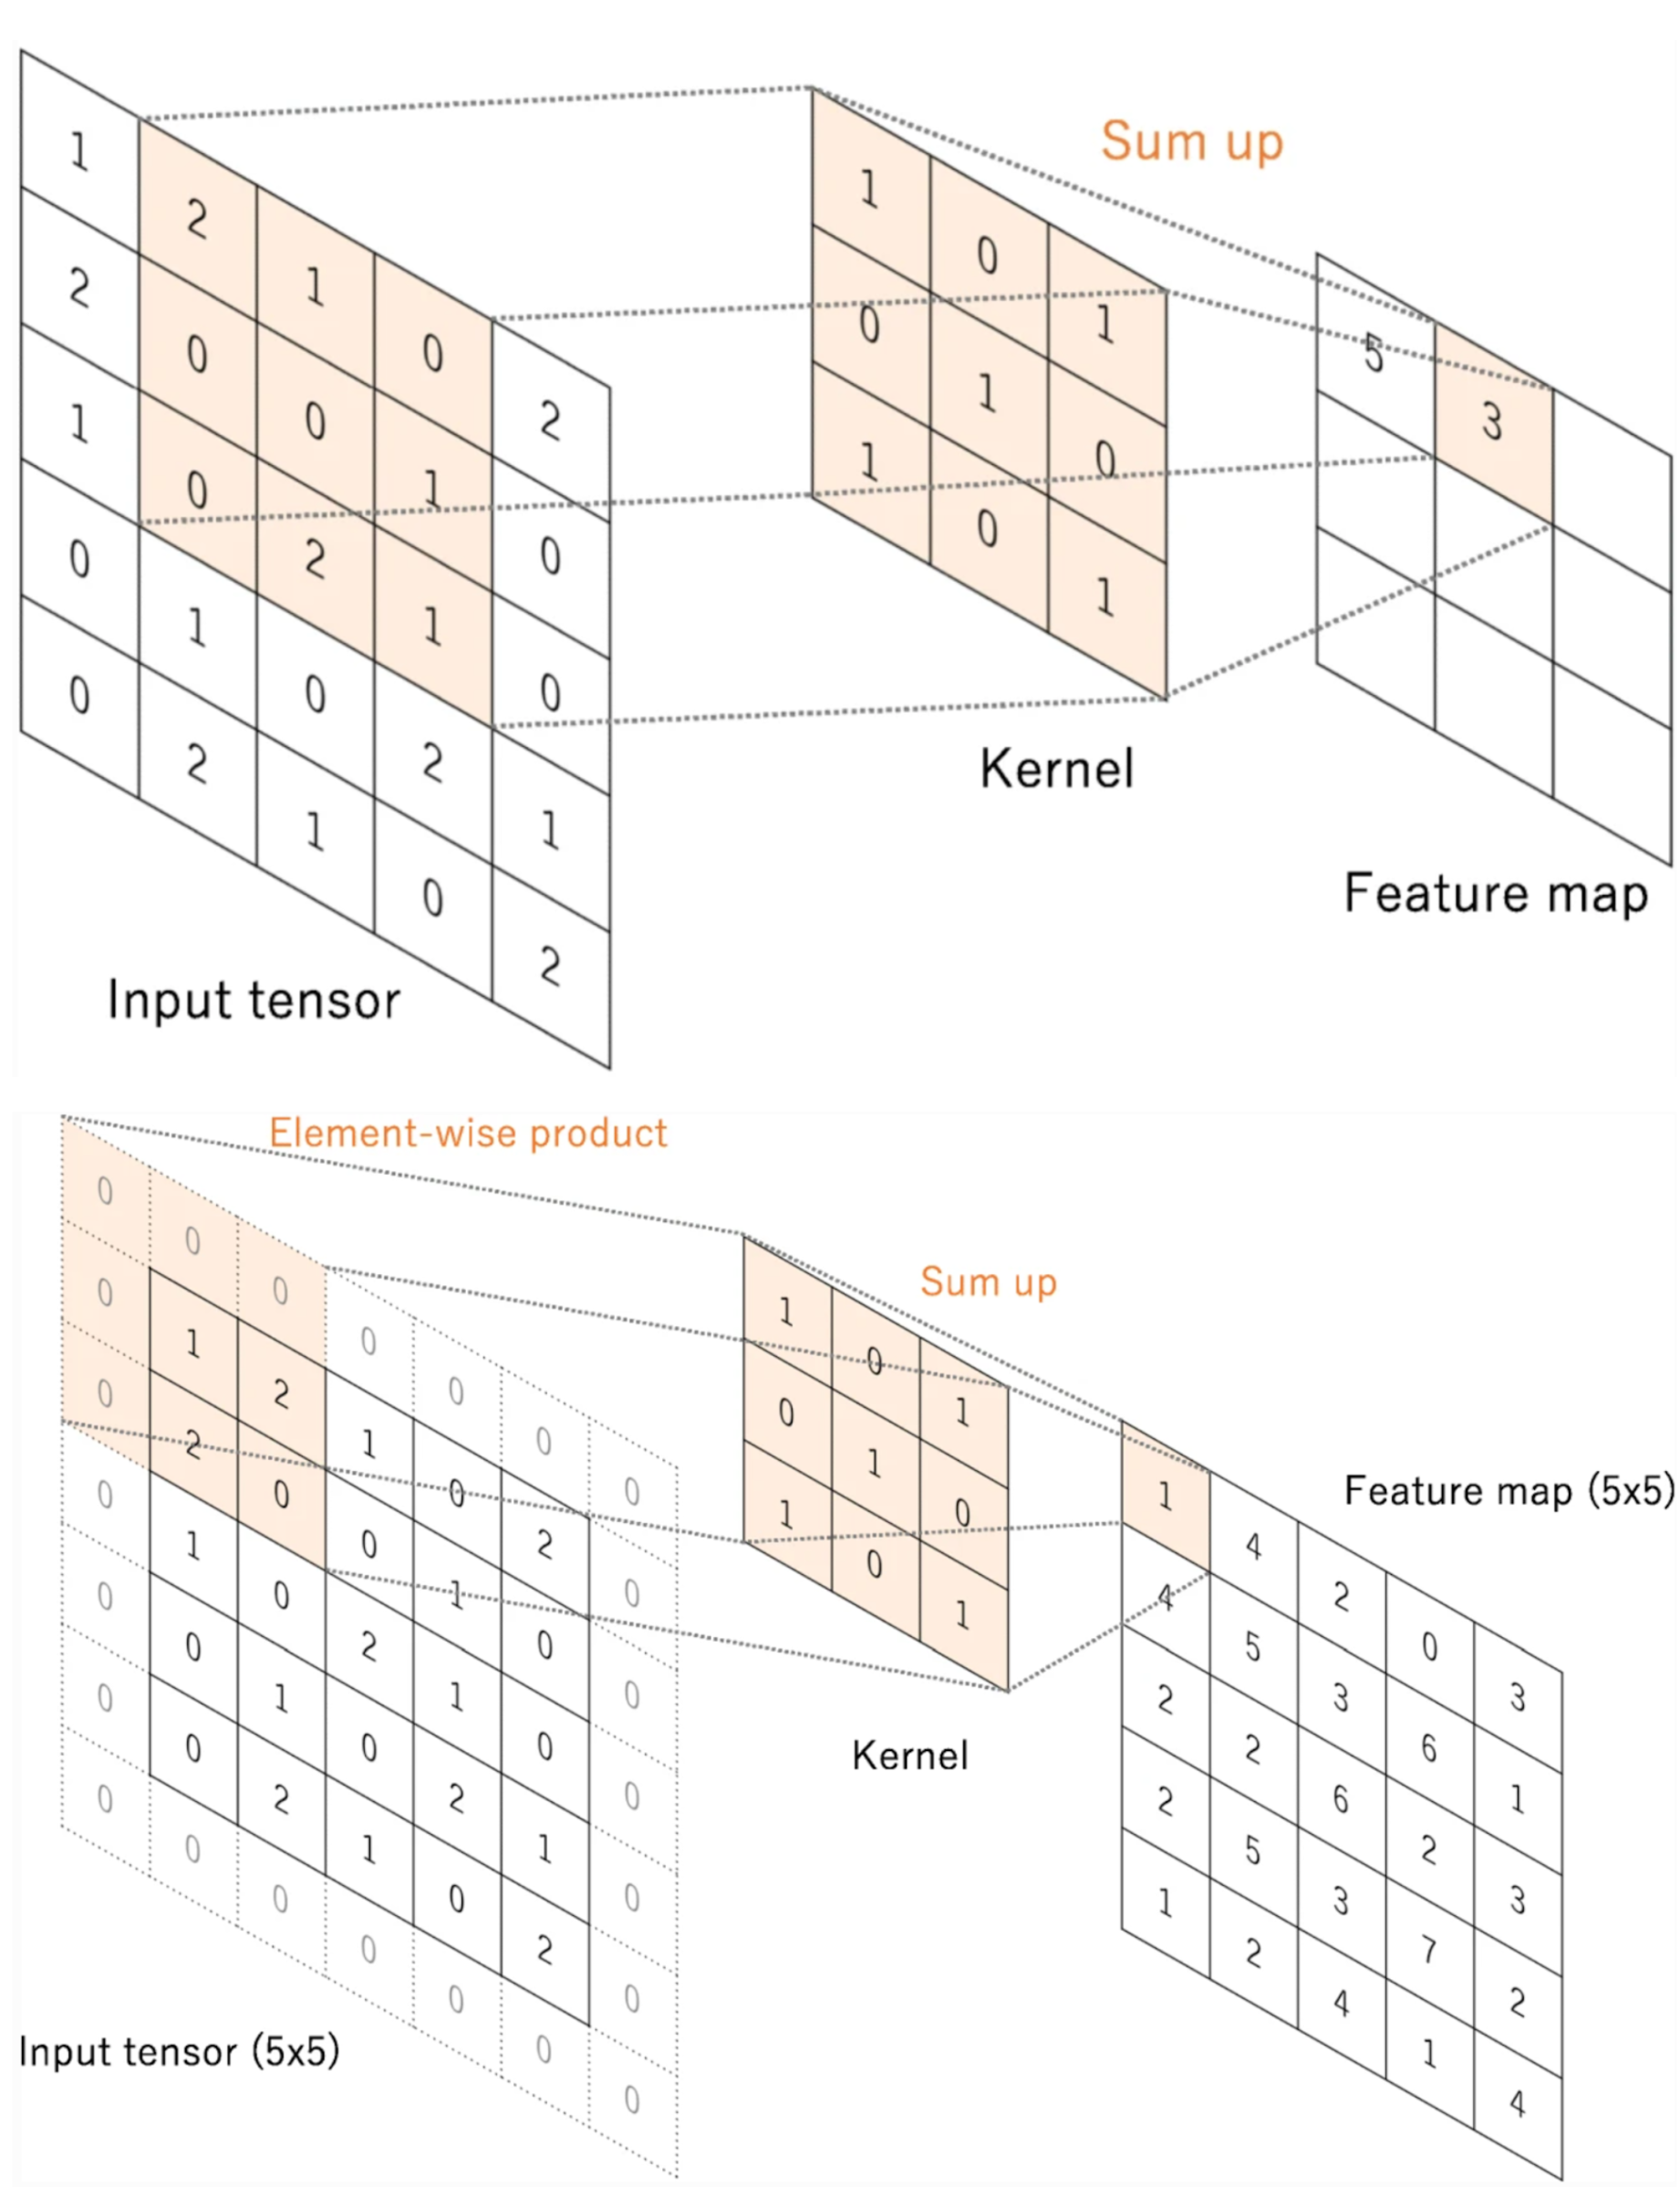
\includegraphics[width=0.5\textwidth]{figures/fig3.png}}
\caption{\label{fig:fig3} An example of a convolution operation with a kernel size of 3×3, an input tensor with no padding on the top and the tensor with padding on the bottom (\cite{yamashita_2018_convolutional}).}
\end{figure}

\subsection{Convolution and activation function}
The first layers are crucial in the feature extracting process (\cite{yamashita_2018_convolutional}). It is a two-step process, where firstly, a convolution operation is performed, followed by an activation function. Convolution is a linear operation performed to extract features from an image. Throughout the process, a kernel, a small array of numbers, is applied through an input array of numbers called an input tensor. After this procedure, the feature map is created (Fig. \ref{fig:fig3}). It can be observed that the outermost rows and columns are being left out of the process, and the information from border pixels is lost. However, a technique called padding can be used to address the issue. Through this process, rows and columns of zeros or mirrored values are added to the input tensor so that the values on the edges are not missed out. 
\\ Nonlinear activation functions are significant to ease the process of training (\cite{ramachandran_2017_searching}). It is being applied to the feature map after the convolution. Rectified Linear Activation function (ReLU) has been one of the most widely applied activation functions due to its effectiveness and simplicity. Each of the numeric pixel values in the feature map is redefined by the following function: \[ f(x) = max(0, x) \] The function will directly output the input in case it is positive and 0 otherwise. 

\subsection{Max pooling}
Max pooling is a pooling operation where, depending on the length of a stride, the input feature map is being downsampled by the maximum value of each MxN group of numbers. All the other values in a patch are disregarded. The most common pooling filter would be a 2x2 filter with a stride of 2, that can be found in Fig. \ref{fig:fig4}.

\begin{figure}[H]
\centering 
\makebox[\columnwidth]{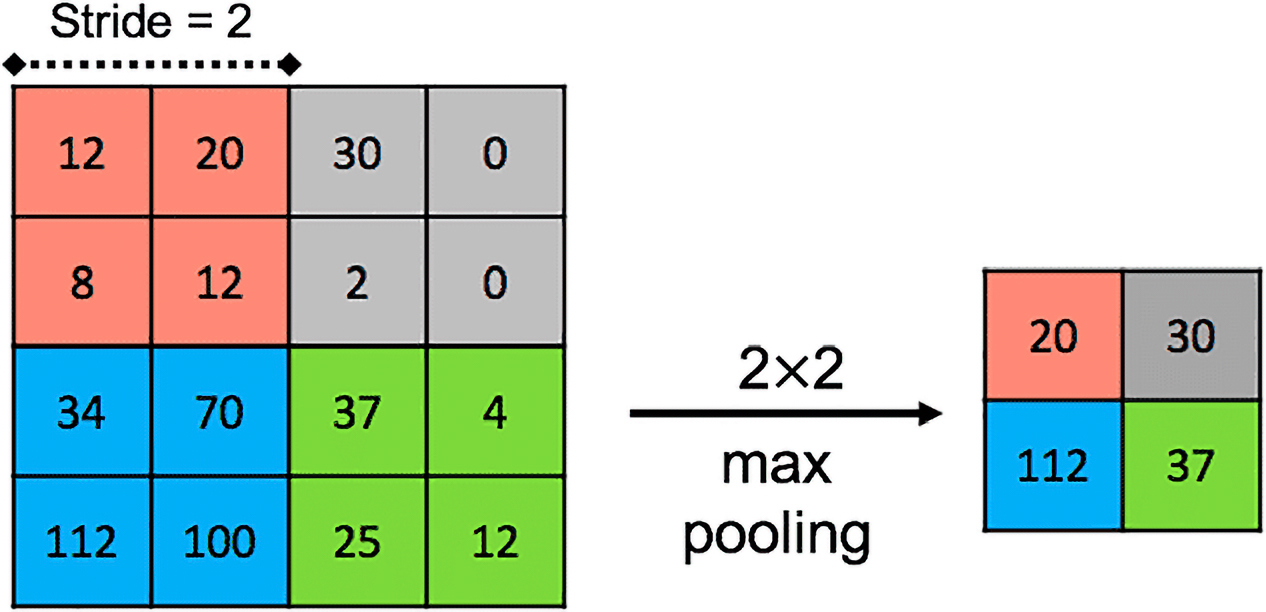
\includegraphics[width=0.5\textwidth,keepaspectratio]{figures/fig4.jpg}}
\caption{\label{fig:fig4} An example demonstrating the process of max pooling  (\cite{gupta_2018_deep}).}
\end{figure}


\section{Approach}
This project aims to create photo/video effects for portrait imagery. The approach to problem-solving is divided into two sections. Firstly the person is segmented out from the background; then, the obtained segmentation masks are used to create the effects. 
Convolutional Neural Networks, specifically CNN with the U-Net architecture, have been used to achieve the solution of the first sub-task.

\subsection{U-Net architecture}
In 2015, Olaf Ronnenberg, Philipp Fischer, and Thomas Brox published a report introducing a new and more efficient architecture for semantic segmentation. Although this convolutional network was initially aimed at biomedical applications, it has been widely used in other areas due to its training efficiency and results. 
The architecture is called U-Net, and an example is presented in Fig. 5. With this architecture, the process is divided into two parts: the contracting path on the left side and the expansive path on the right side of the image.

The contracting path follows a traditional convolutional network architecture. Firstly 3x3 unpadded convolutions are applied two times; a ReLU activation function is applied after each application. It can be observed that the image resolution decreases by two from both the height and the width after each convolution. It is due to the lack of padding. Next, a 2x2 max pooling operation with stride two is executed on the layer, thus downsampling the image. The feature channels are doubled after each downsampling procedure. 
In the bottom row of Fig. 5, where it is a 32x32 pixel image left with 1024 feature maps, up-convolution is applied to upscale those.

\begin{figure}[hbt]
\centering 
\makebox[\columnwidth]{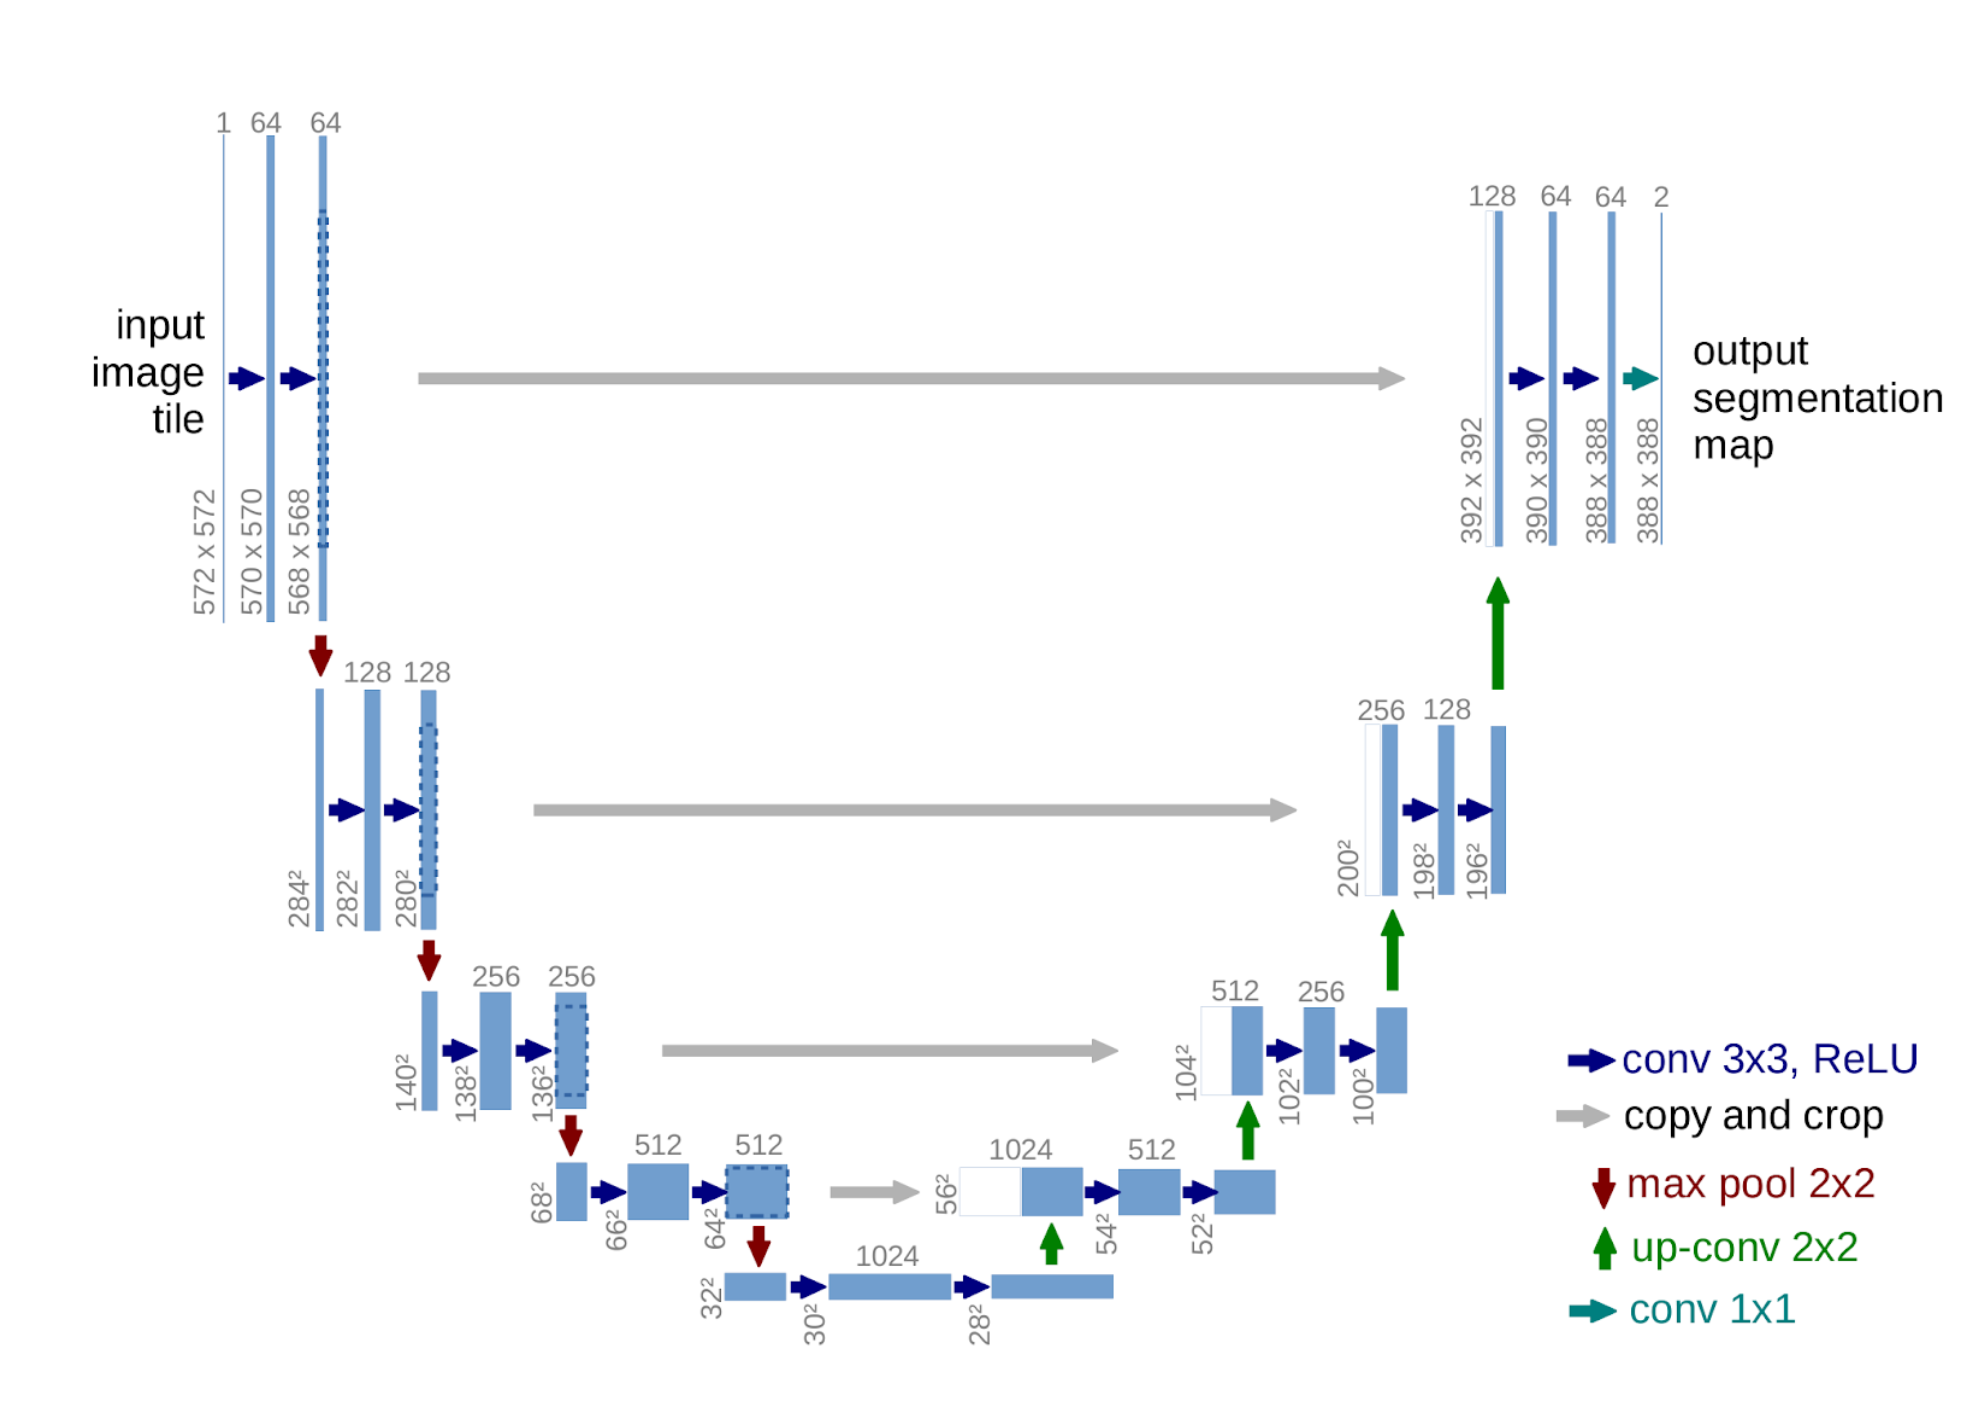
\includegraphics[width=0.5\textwidth,keepaspectratio]{figures/fig5.png}}
\caption{\label{fig:fig5} U-Net architecture example. The blue boxes represent a multi-channel feature map. The white box represents a copied feature map. The arrows represent the convolution operations happening on different layers and the application of the ReLU activation function (\cite{ronneberger_2015_unet}).}
\end{figure}

The feature map channels are up-sampled on each up-convolution layer and are concatenated with the cropped feature maps from the equivalent line on the contracting path. Cropping is necessary due to the loss of border pixels on each convolution. The final stage of the expansive path is running a 1x1 convolution to map all the feature maps into multiple layers of classes (2 in the case of Fig. \ref{fig:fig5}).

\subsection{Effects}
Multiple effects have been implemented on the images after the segmentation process. One significant advantage of person segmentation is that the effect can be applied separately to either background or the person. 

\begin{figure}[H]
\centering 
\makebox[\columnwidth]{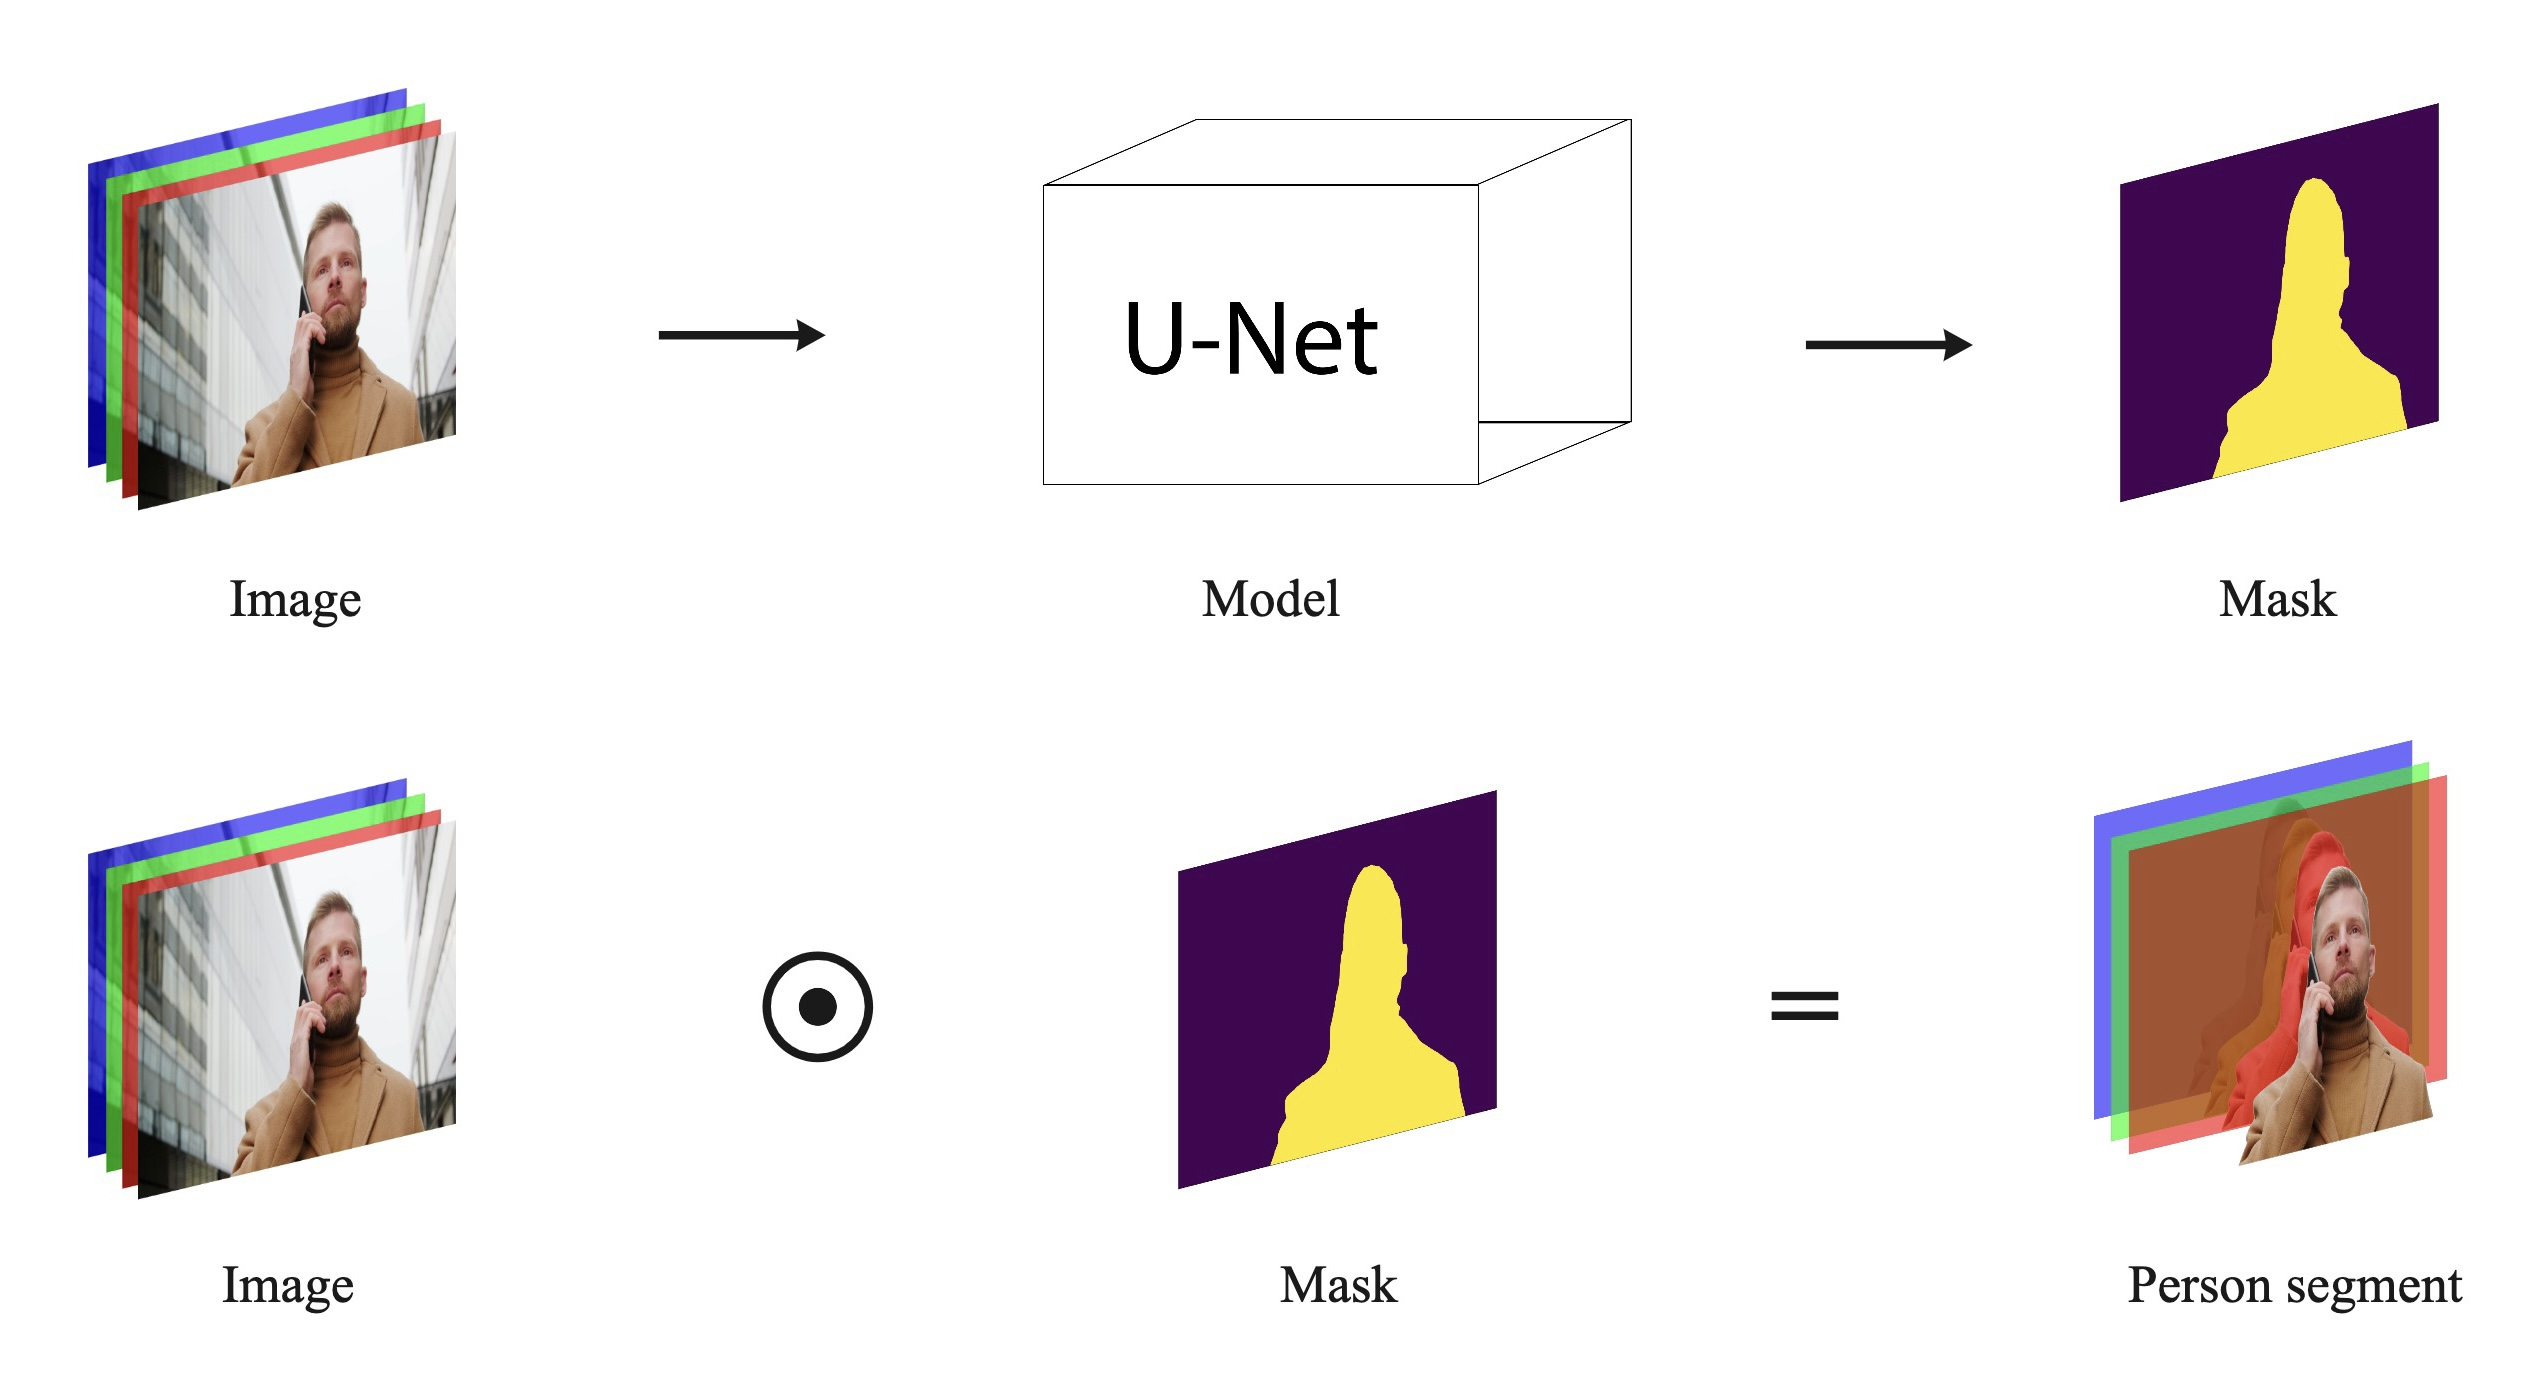
\includegraphics[width=0.5\textwidth,keepaspectratio]{figures/graph1.jpg}}
\caption{\label{fig:graph1} Background removal: execution process.}
\end{figure}

\subsubsection{Background removal}
Person segmentation can effectively be used to manipulate the background of an image.
The image is loaded and resized to go through the model. The resulted binary mask is multiplied with the original image to create a person segment later on, as presented in Fig. \ref{fig:graph1}.

\begin{figure}[H]
\centering 
\makebox[\columnwidth]{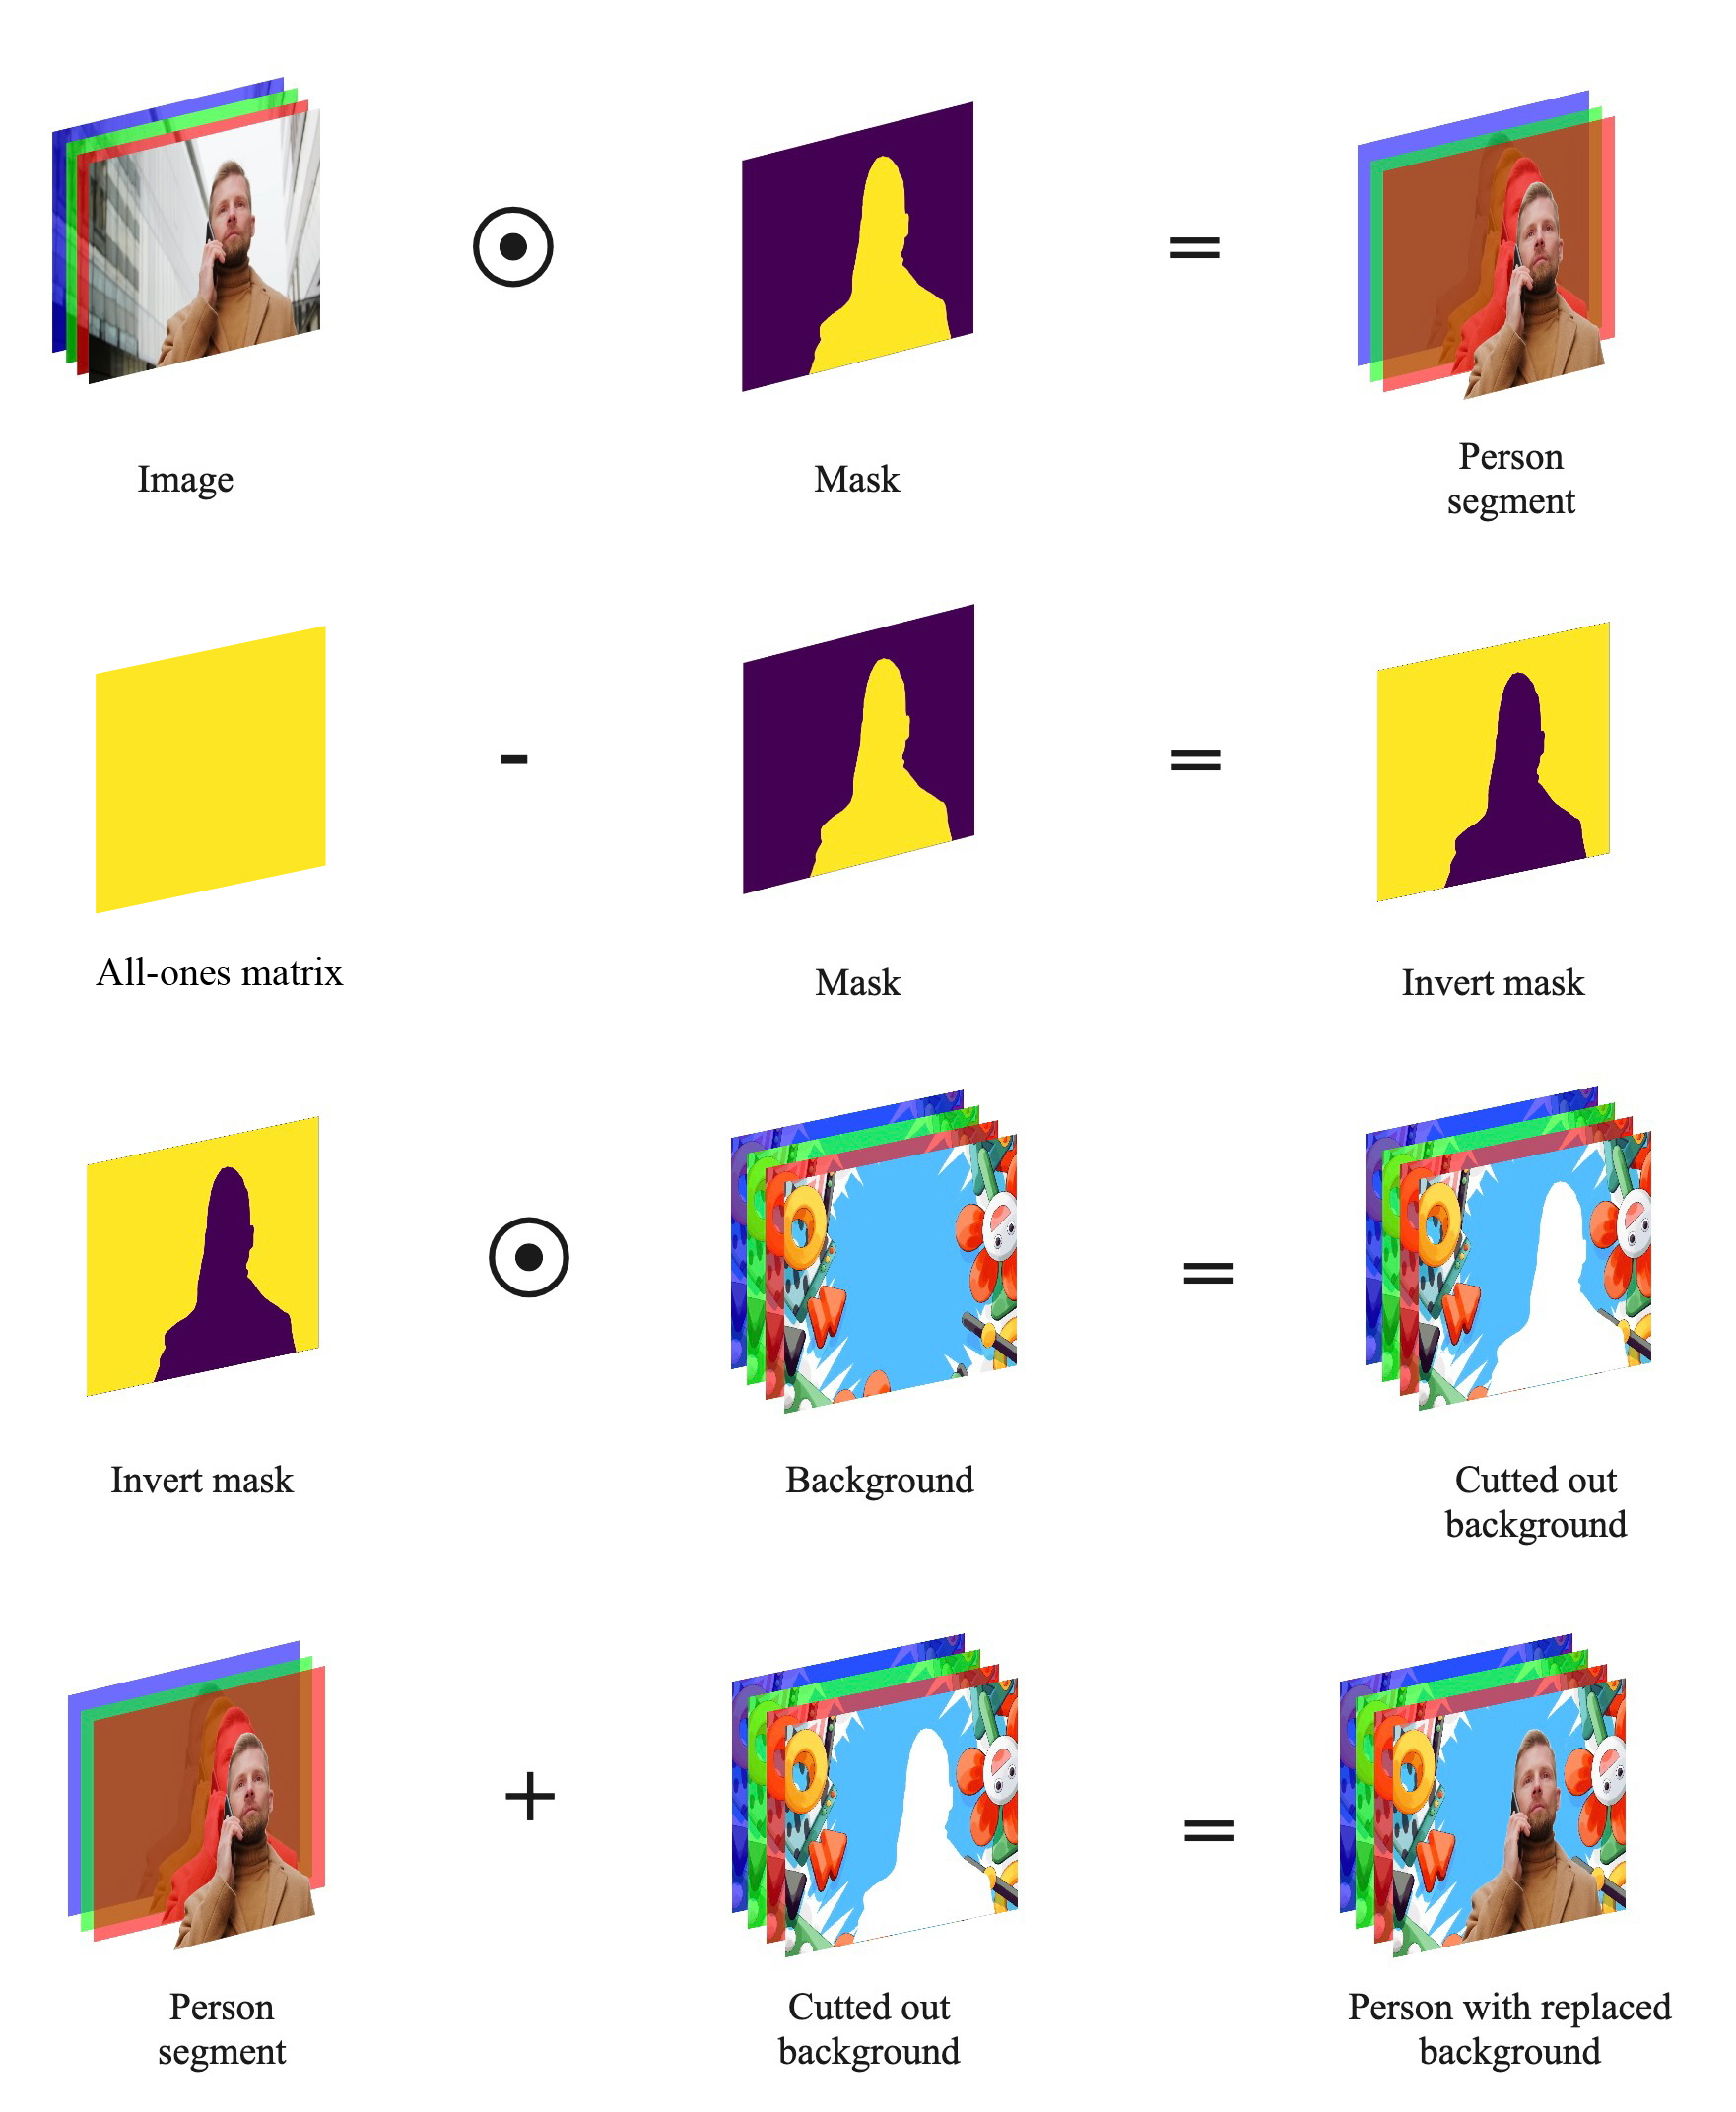
\includegraphics[width=0.5\textwidth,keepaspectratio]{figures/graph2.jpg}}
\caption{\label{fig:graph2} Background replacement effect: execution process.}
\end{figure}

\subsubsection{Background replacement}
The background replacement takes the already segmented person as an array, and according to the size of the input image, resizes the background image and automatically crops to fit in with the aspect ratio of the input image (Fig. \ref{fig:graph2}).


\subsubsection{RGB glitch effect}
The following effect is created by splitting the image color channels into separate red, green and blue channels and moving those along the axis of the image's canvas (Fig. \ref{fig:graph3}). After person segmentation, the output portrait image has been split into red, green, and blue channels. Padding has been added to two color channels only, 5\% from the top and 5\% from the left side, respectively. The padded channels have later been cropped to match the initial image resolution and finally merged back together.

\subsubsection{Person outline}
For this effect, the binary mask created by the model was taken, and applied to the blue channel of an image with with RGB channel with values of zeros (a plain black image with the resolution of the mask), an OpenCV function, contour detection, was applied to detect the edges between the person and the background, that will become the outline later (Fig. \ref{fig:graph4}). The result of the function is a matrix with the position values of the outline pixels. These values are used to draw an outline on an image by replacing the pixels in the original photo.

\begin{figure}[hbt]
\centering 
\makebox[\columnwidth]{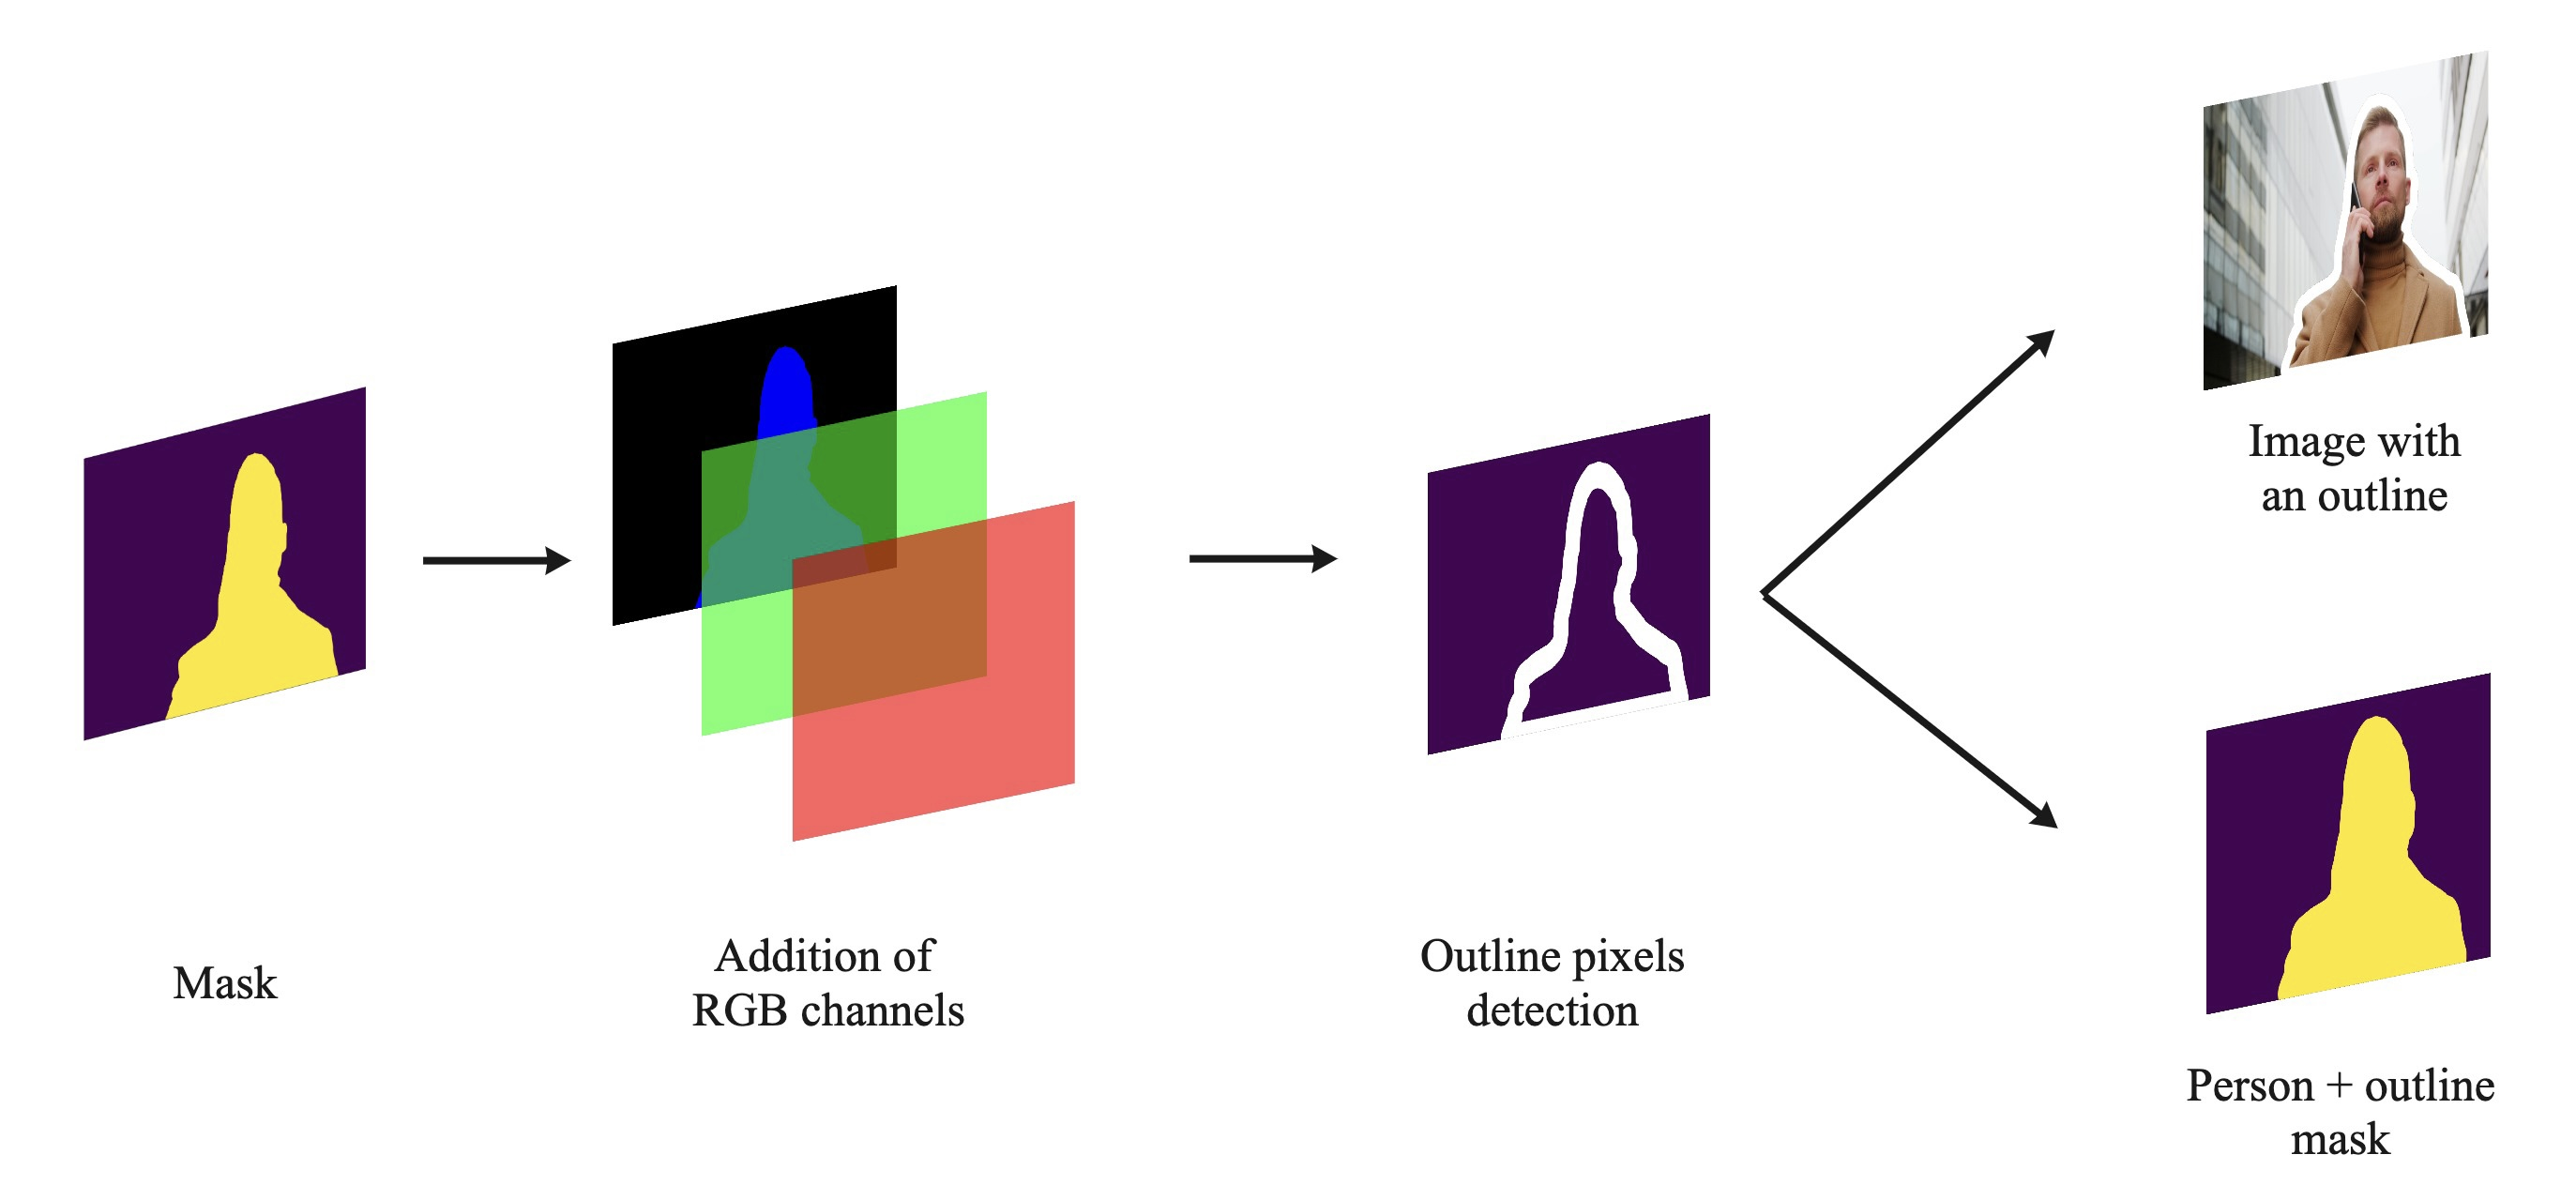
\includegraphics[width=0.5\textwidth,keepaspectratio]{figures/graph4.jpg}}
\caption{\label{fig:graph4} Person Outline effect: execution process.}
\end{figure}

\section{Model training and evaluation}
The data has been collected from Kaggle, a platform to access public datasets and explore different models. The dataset consists of 18,500 samples of portrait images for training and 3,500 portraits for testing. Due to the small size of the images, 128x128 pixels, the training happened in a relatively short time. The image size has been selected to be 128x128, due to lack of computing power. Thus, the results are expected to be less accurate than those present in the source. 
Initially, the training and test sets have been prepared for training. The segmentation-models library has been used to access the predefined architecture of the U-Net model in python. 

\begin{figure}[hbt]
\centering 
\makebox[\columnwidth]{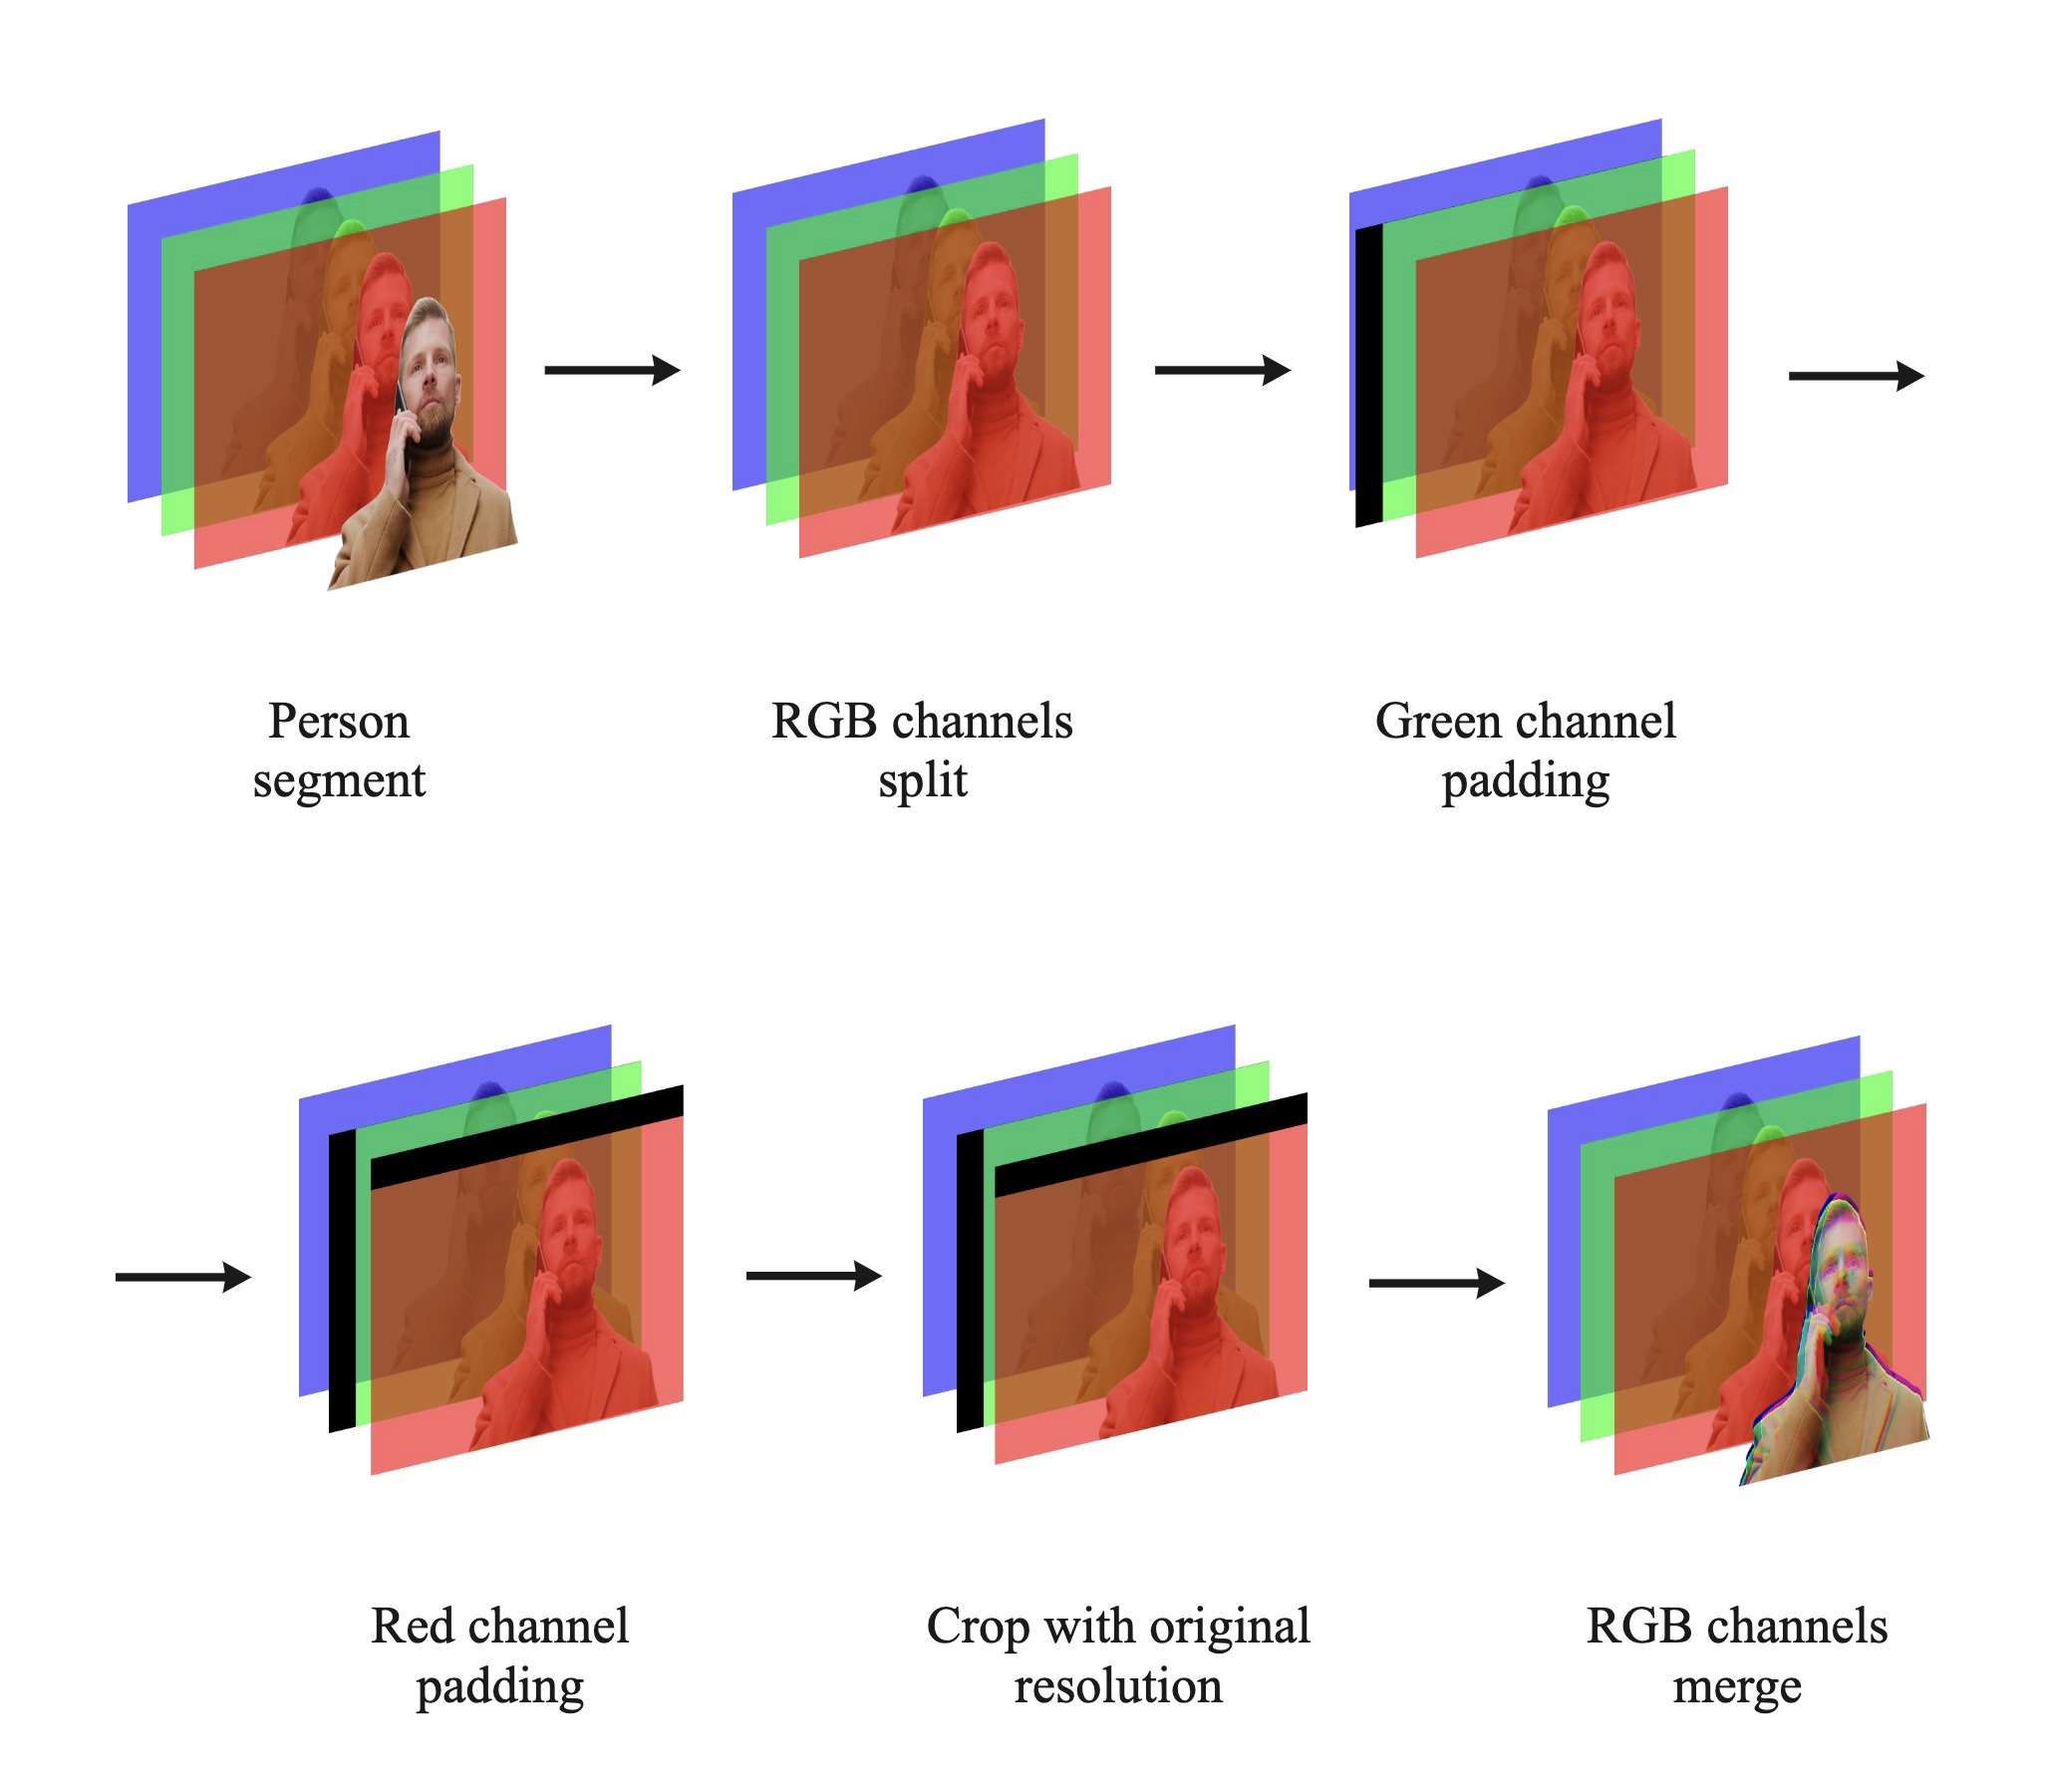
\includegraphics[width=0.5\textwidth,keepaspectratio]{figures/graph3.jpg}}
\caption{\label{fig:graph3} RGB Glitch effect: execution process.}
\end{figure}

A Jaccard loss function have been defined to measure the efficiency of the model (Eq. \ref{eqn}). 

\begin{equation} 
\label{eqn}
Jaccard(A,B) = \frac{|A\cap B|}{|A\cup B|}
\end{equation}

This function, also known as intersection-over-union (IoU) loss, evaluates the segmentation quality by dividing the intersection and the union of two sets, A and B. The values of the coefficient vary between 0 and 1. The former represents zero if the sets are disjoint, and it is one if they are identical (\cite{duquearias_2021_on}). In our case, the intersection is the overlap area of the prediction and the ground truth image, and the union is the union between those two areas.

The Adaptive Moment Estimation Algorithm (ADAM) has been selected as an optimization algorithm. It is much more efficient than the gradient descent or stochastic gradient descent methods (\cite{battini_2018_adam}). It is easy to implement, does not require much memory, and works well with large datasets.

\section{Results}
Three types of effects have been created through this project using semantic segmentation. The images that are presented in the following figures  (Fig. \ref{fig:fig6}, \ref{fig:fig7}) are selected to be close-up portraits with neutral/mono-color background, and the results are close-to pleasing. 
The model training has been executed for five epochs with a batch size of 64 images. The IoU score after the fifth round of training has been 0.9648, meaning that the prediction mask is approximately 96.5\% accurate. Compared to the results in the source of segmentation technique, however, we have got a lower IoU score: 0.9648 vs. 0.981. The difference might be because of the lower number of epochs run in our case. In the original study, the training was run for ten epochs. However, it is five within the scope of this project. 
The model has been tested for images with multiple people on it; however, it performs better when only one person is on the image. Also, as the training dataset consisted of mostly close-up portraits, the model performs poorly when applied to the whole body. 
In addition, the model was run on the test set of the database to calculate the mean and the median time of the model execution per frame. The data was adjusted for outliers by keeping the values up to two standard deviations away from the mean. Table \ref{tab:table1} was created by running the model on the test set of images of approximately 4000 images. According to our results, the mean execution time per frame was 0.077 seconds, and the median was 0.073 seconds. These numbers indicate that to run the model on 1 second of footage will take 2 seconds on average. If the frame rate is 25 frames per second (FPS), in case FPS is higher, more time will be required to execute a one-second video. Whenever the image resolution increases, we can observe a significant increase in the execution time of semantic segmentation per frame to approximately 0.15 seconds in the case of 256x256 images and around 0.54 seconds per 512x512 pixel resolution image. The results might improve if the model is trained on resolutions higher than 128x128 pixels.


\begin{table}[H]
\centering
\caption{Per-frame execution time}
\begin{tabular}{cccl}
\textbf{Resolution (px.)}     & \textbf{Mean value (sec.)}    & \textbf{Median value (sec.)}  &   \\
\\
\hline
\textbf{128x128}              & 0.077                & 0.073                &   \\
\textbf{256x256}              & 0.15                 & 0.147                &   \\
\textbf{512x512}              & 0.545                & 0.538                &   \\
\hline
\multicolumn{1}{l}{} & \multicolumn{1}{l}{} & \multicolumn{1}{l}{} &   \\
\multicolumn{1}{l}{} & \multicolumn{1}{l}{} & \multicolumn{1}{l}{} &  
\label{tab:table1}
\end{tabular}
\end{table}


The results of our background removal process are depicted in Fig. \ref{fig:fig6}. It can be observed that the output images have got lower resolution than the original images. This is because the model was trained on 128x128 images, and thus the resolution of the images suffered significantly.

\begin{figure*}[hbt]
\centering 
\makebox[\columnwidth]{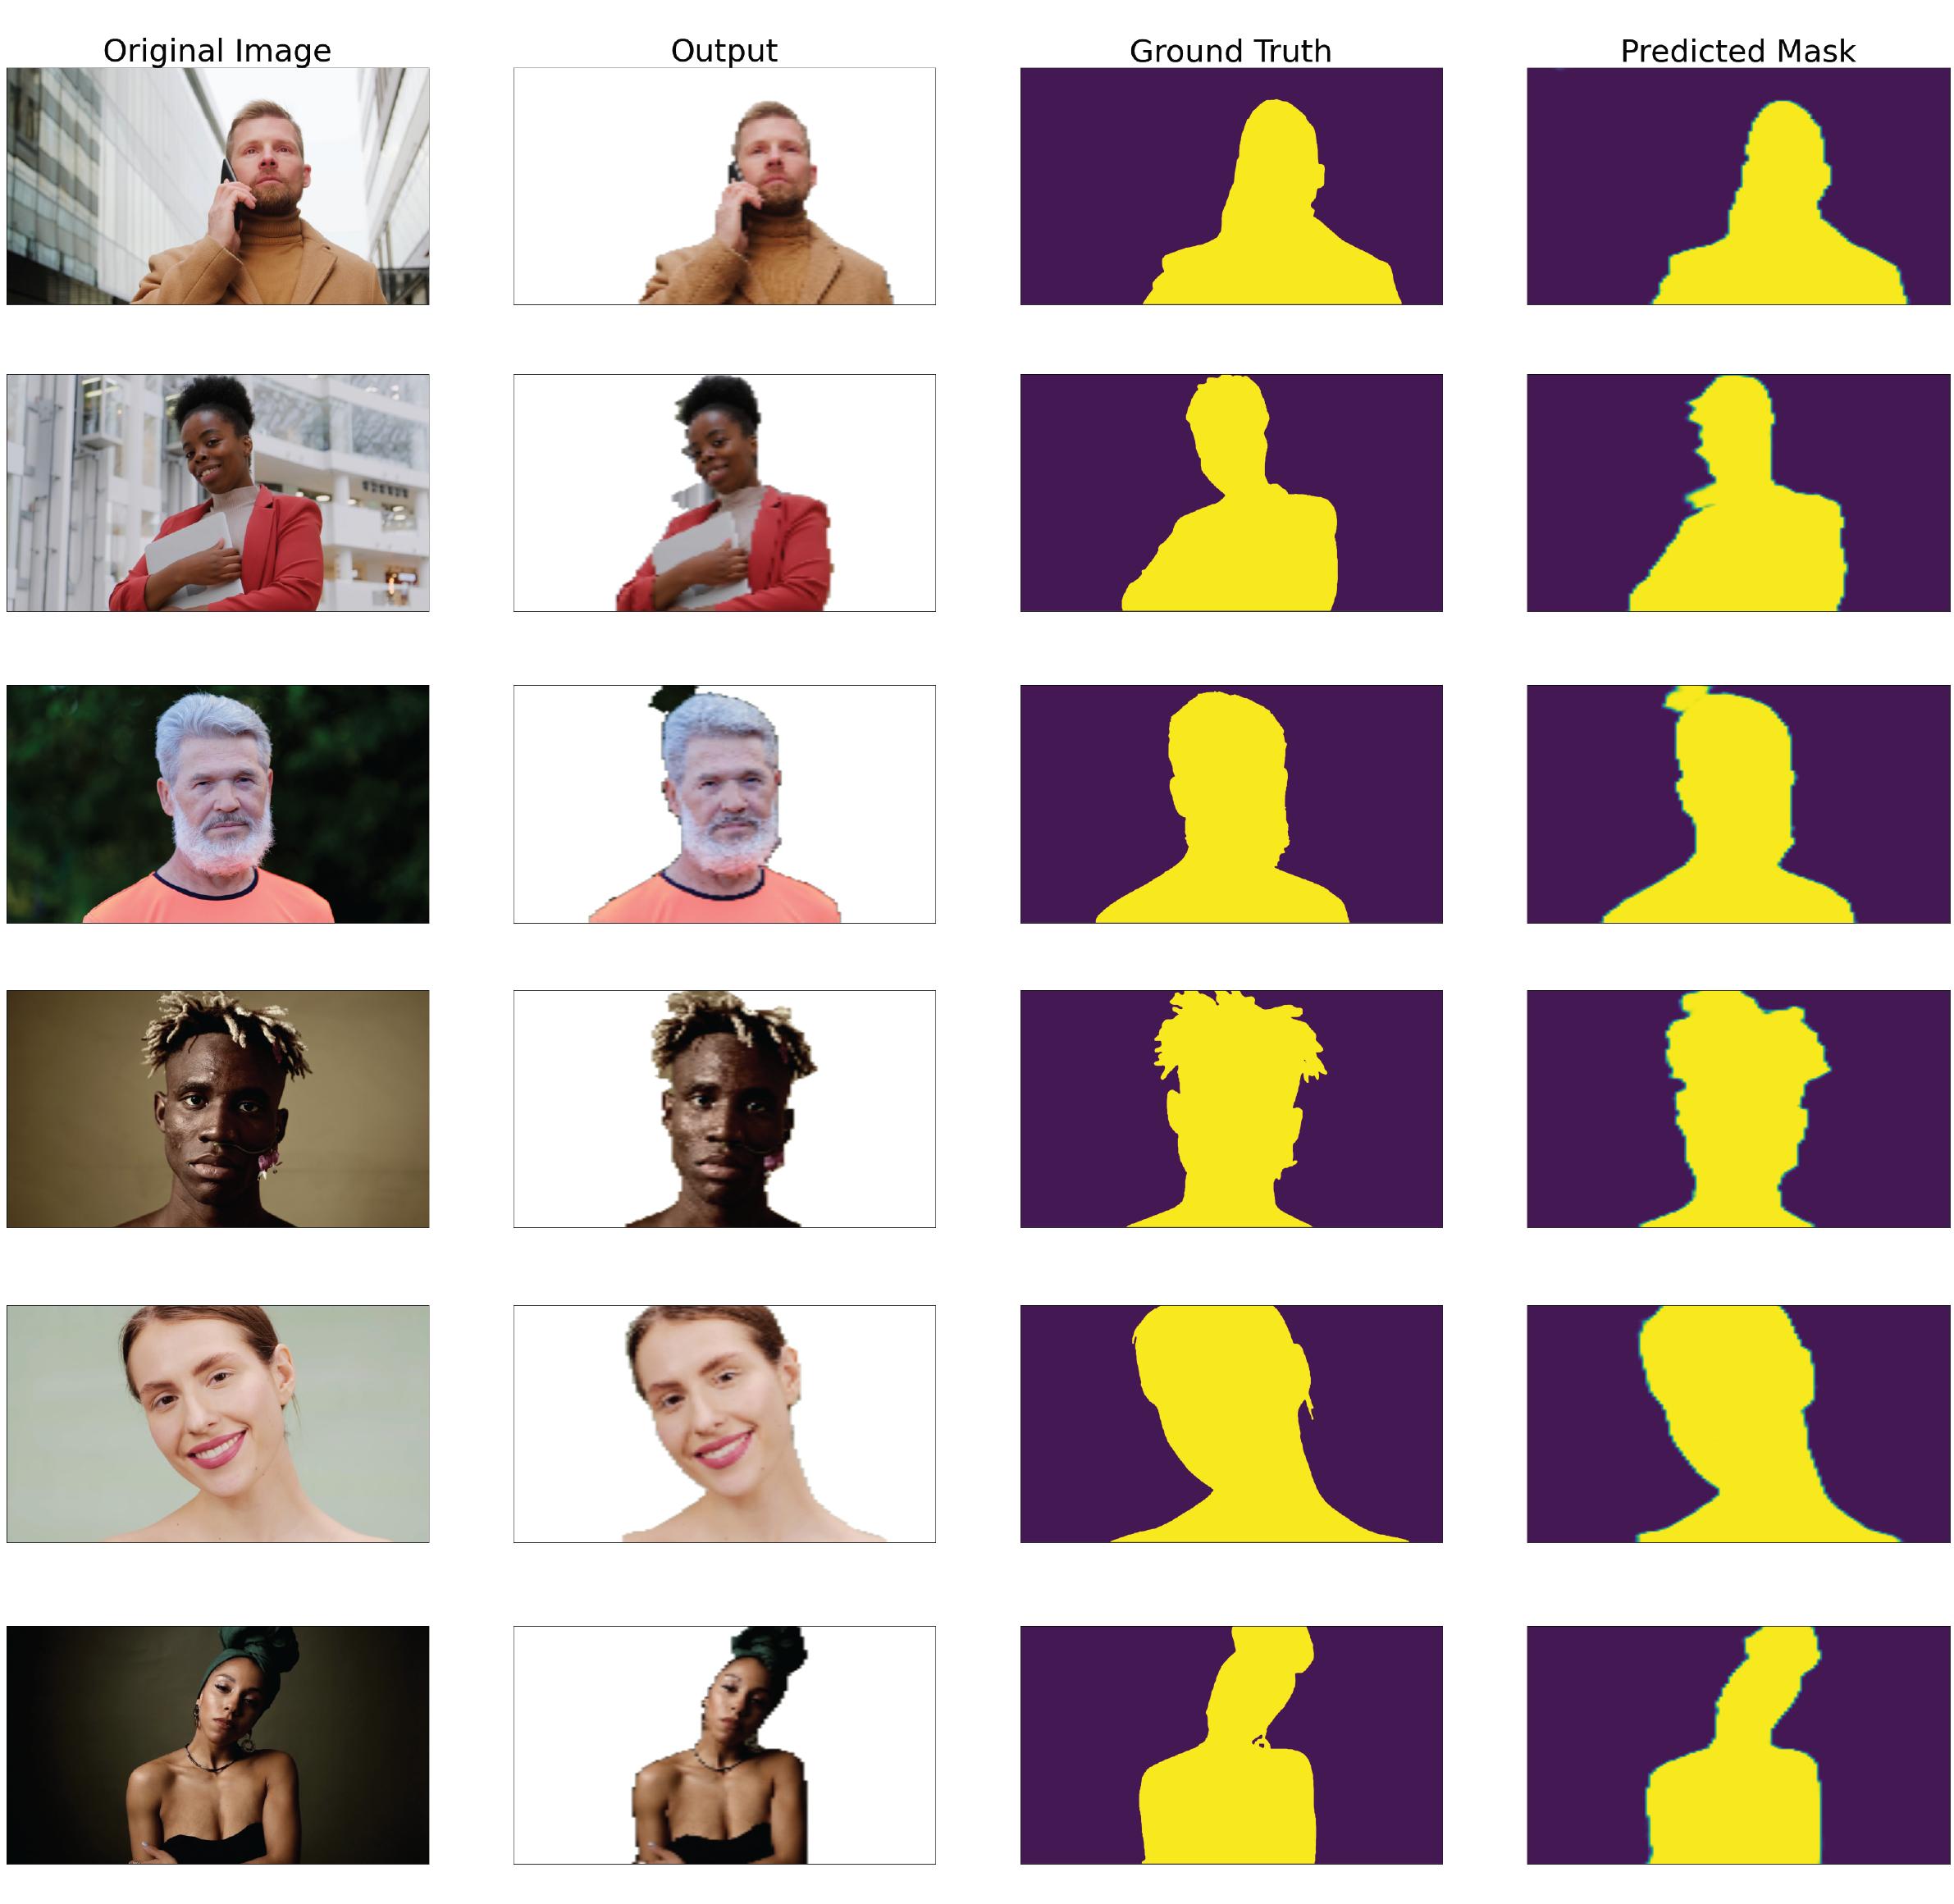
\includegraphics[width=0.9\textwidth,keepaspectratio]{figures/fig6.png}}
\caption{\label{fig:fig6} Background removal results: Original images in the first column, the segmented person in the second column, ground truth mask in the third column, and the predicted mask by our model in the fourth column.}
\end{figure*}

Fig. \ref{fig:fig7} represents the results of the background replacement, RGB glitch and the person outline effects. Persons are segmented out from the images, and then the background is replaced with a given image. One major drawback is that the color grading of the person and the background do not match perfectly. Thus another effect could have been added to the final result to merge the colors of the background and the person so that it looks less artificial. Overall if the portrait segmentation is improved, the results of this effect would improve significantly.

\begin{figure*}[hbt]
\centering 
\makebox[\columnwidth]{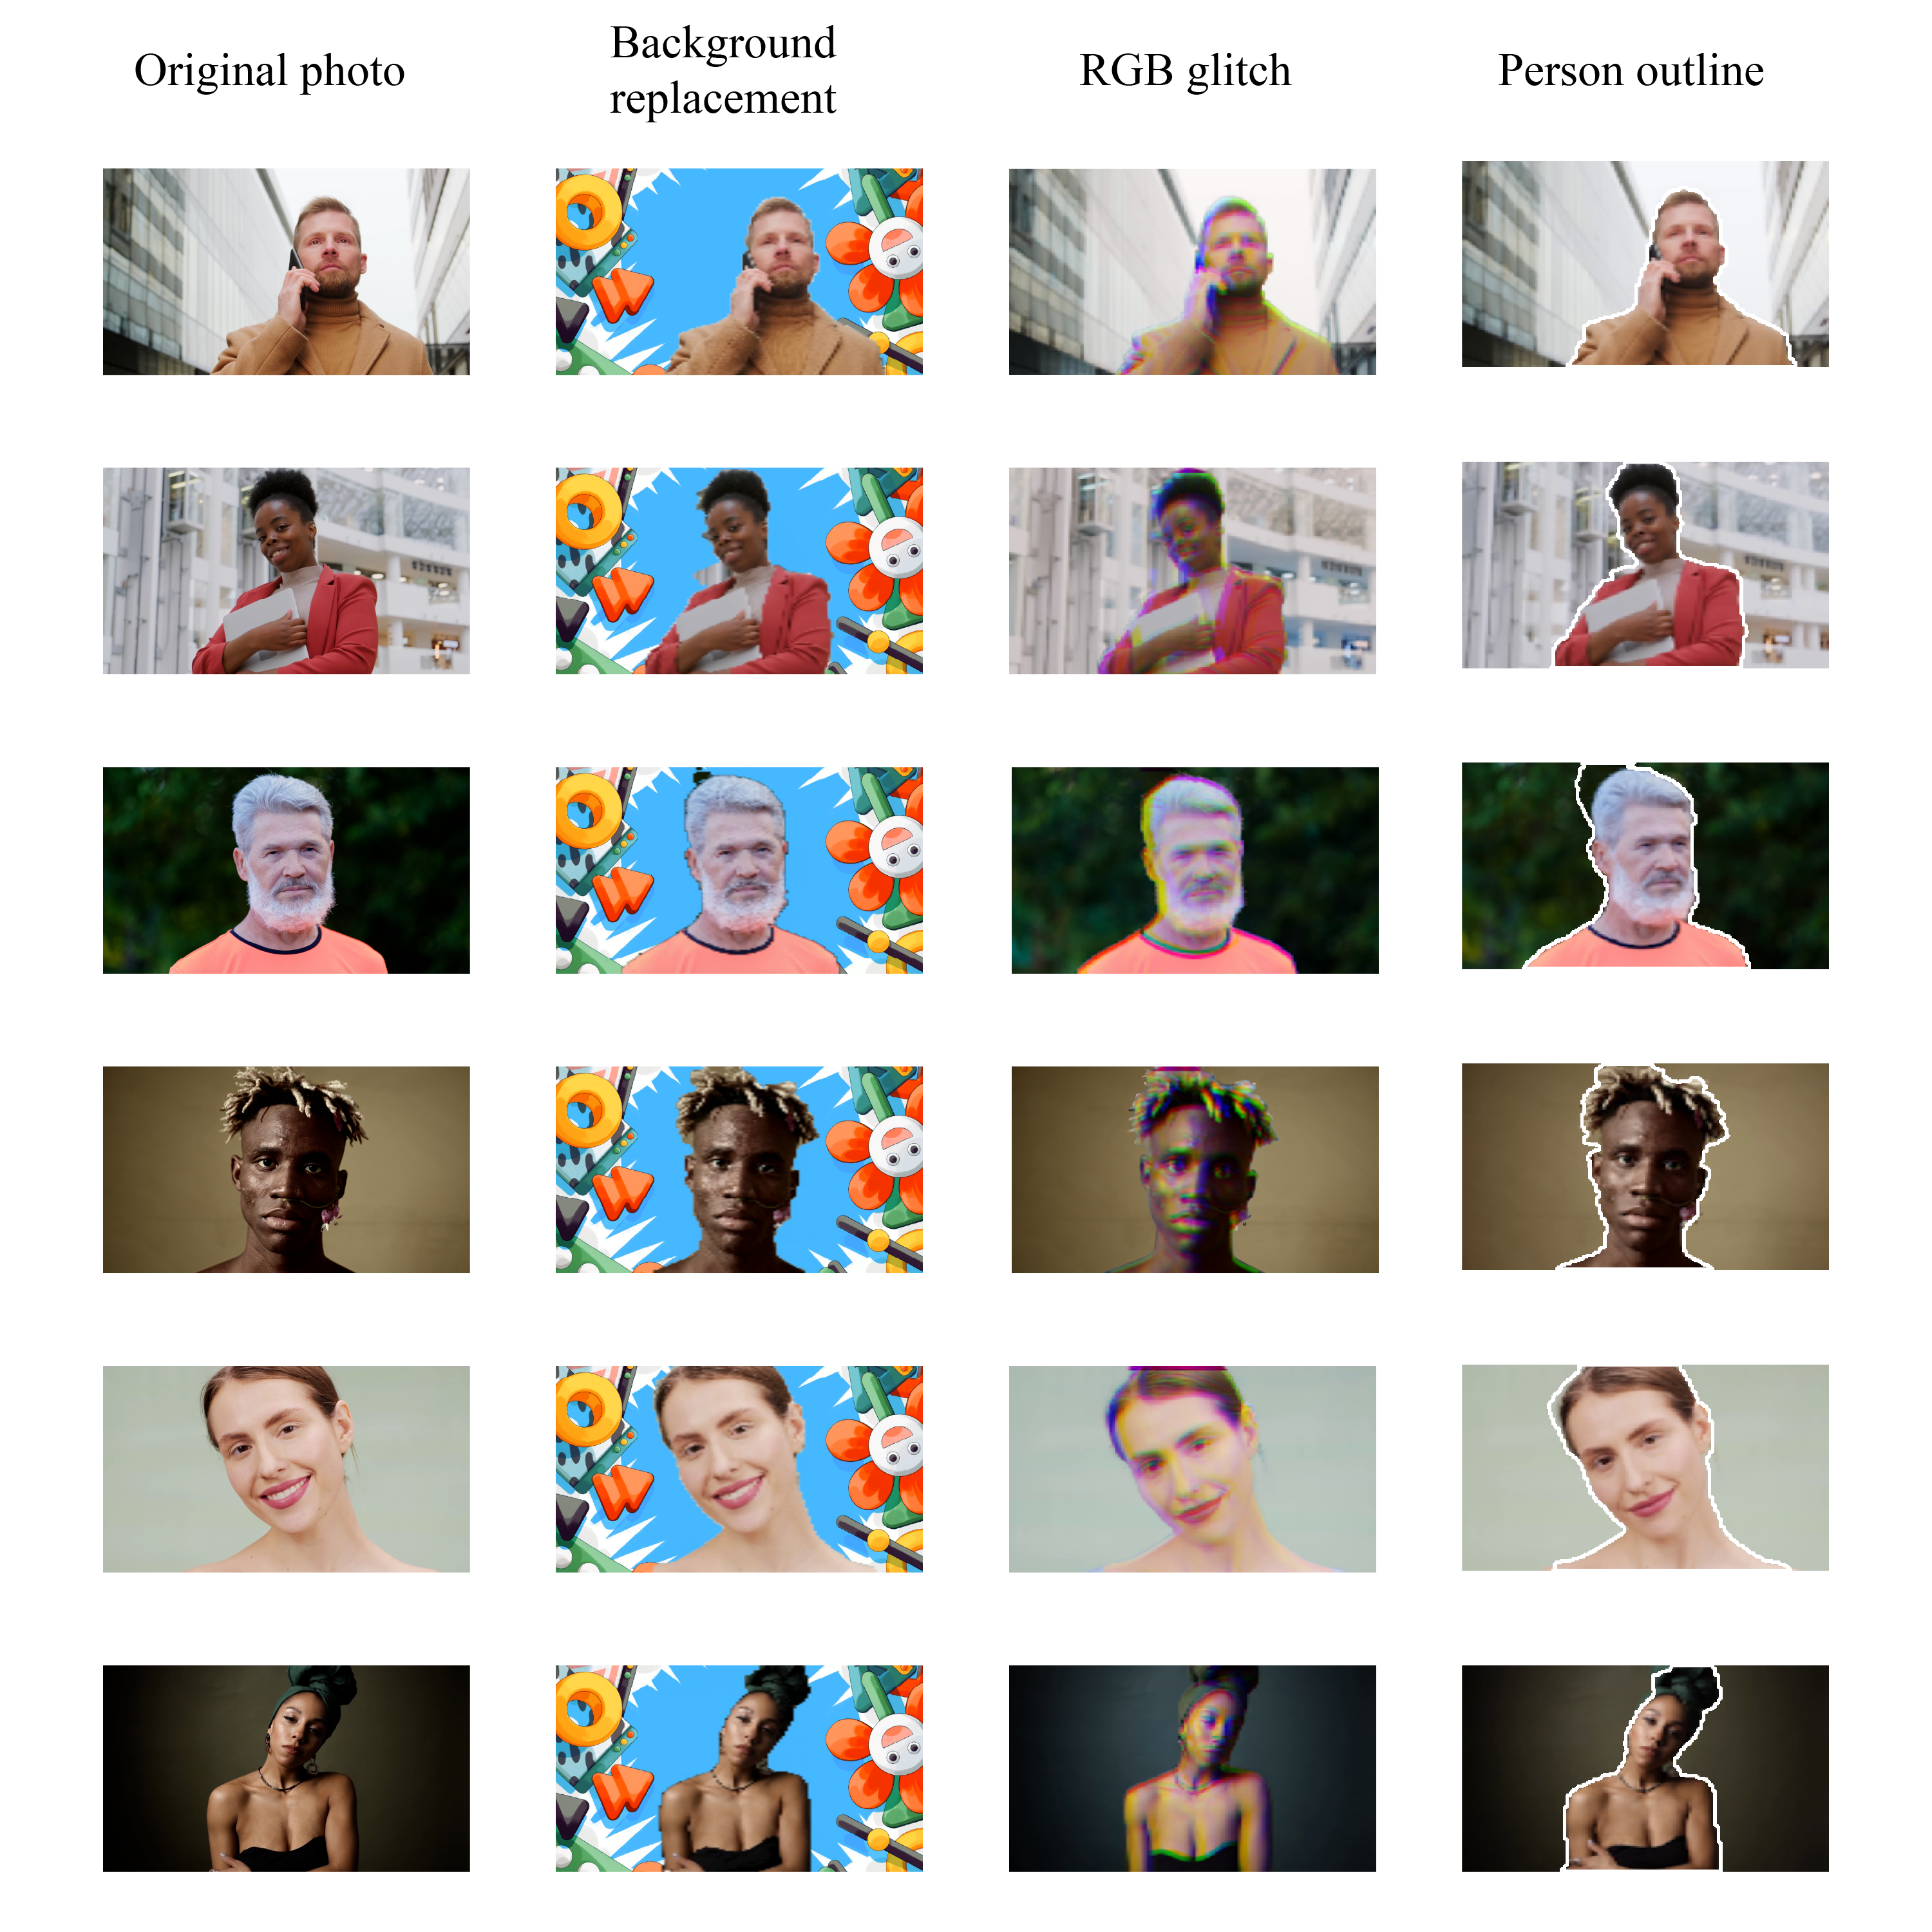
\includegraphics[width=\textwidth,keepaspectratio]{figures/Fig7.png}}
\caption{\label{fig:fig7} Photo/Video effects results: Original images in the first column, background replacement effect in the second, RGB glitch in the third, and person outline in the fourth column.}
\end{figure*}


\section{Conclusion and Future Work}
In the framework of this project, photo/video effects have been applied to portrait imagery/video based on semantic segmentation. The way person segmentation was done was by using convolutional neural networks. After the training, we separated the person from the background and applied the background replacement, RGB glitch, and person outline effects on the person segment. 

To improve the results further, we recommend running the model training on at least 512x512 resolution images to have a higher resolution output. In order to produce better visual results further training should be performed on images that include full-body shots from a distance and multiple people. 
\clearpage
\printbibliography

\end{document}